% Chapter 2
%----------------------------------------------------------------------------------------
\chapter{Marco Teórico} % Main chapter title
\label{Chapter2} % For referencing the chapter elsewhere, use \ref{Chapter2} 
\begin{onehalfspacing}
%----------------------------------------------------------------------------------------
%
%
%----------------------------------------------------------------------------------------
%SECCIÓN 2.1 
%----------------------------------------------------------------------------------------
%
%
\section{Detección de Mentiras}
\label{sec:Deteccion_de_Mentiras}
%----------------------------------------------------------------------------------------
En la literatura se menciona que en principio existen tres maneras de poder detectar mentiras en un individuo. La primera forma es observando cómo se comportan; en esta parte se analizan los movimientos corporales, si la persona sonríe, si desvía la mirada, la intensidad de la voz, rapidez del discurso, entre otros. La segunda forma es escuchando qué es lo que están diciendo, aquí se analiza el contenido del discurso; y la última forma es midiendo las respuestas psicológicas que tiene el individuo \cite{Grubin2005LieReview}.\\

%----------------------------------------------------------------------------------------
\subsection{Detección por lenguaje verbal}
\label{sec:Lenguaje_verbal}

Se pueden evaluar las diferencias entre los mentirosos y los que no mienten, a través de lo que dicen, con el SVA (Statement Validation Analysis). El núcleo del SVA es el CBCA (Criteria Based Content Analysis), una evaluación sistemática de la credibilidad de las declaraciones dichas. CBCA se basa en la hipótesis de que una afirmación derivada de la memoria de una experiencia real difiere al contenido y calidad de una afirmación basada en una invención o fantasía. La presencia de cada criterio refuerza la probabilidad de que lo contado se base en una experiencia personal genuina. En otras palabras, las declaraciones verdaderas se caracterizarán por más elementos medidos por CBCA que por declaraciones mentirosas. De esta manera se puede detectar si una persona miente a través del lenguaje verbal \cite{Vrij2000DetectingBehavior}.\\

%----------------------------------------------------------------------------------------
\subsection{Detección por respuestas fisiológicas}
\label{sec:Respuestas_psicologicas}

El polígrafo es un instrumento sofisticado que se ha utilizado para detectar mentiras midiendo reacciones fisiológicas. Para poder utilizar un polígrafo, los expertos han desarrollado exámenes, procedimientos y técnicas como el CQT (Control Question test) y  GKT (Guilty Knowledge Test) \cite{Staunton2011AnExamination}.\\


El polígrafo moderno creado por John Larson, graba simultáneamente en un papel tres respuestas psicológicas asociadas con mentiras; presión arterial, pulso cardiaco y la respiración. El polígrafo a pesar de ser un instrumento para detectar mentiras, no detecta mentiras; en cambio mide respuestas psicológicas que son asociadas con comportamientos de mentira. La presencia de estas respuestas que “delatan mentira” no necesariamente especifican mentira y no necesariamente se tienen que mostrar cada vez que una persona dice mentiras \cite{Vrij2000DetectingBehavior}. Combinar expertos en mentiras en conjunto con otras técnicas (GKT, CQT) resulta bastante útil para detectar mentiras y el uso de estos instrumentos es apoyada por la policía, seguridad, inteligencia y varios campos clínicos, pero científicos y académicos comentan no confiar en éste instrumento.

%----------------------------------------------------------------------------------------
\subsection{Detección por lenguaje no verbal}
\label{sec:Lenguaje_no_verbal}
Tres perspectivas (la emocional, carga cognitiva y el intento de control de comportamiento) son importantes para detectar mentiras a través del lenguaje no verbal \cite{DePaulo2003CuesDeception}. Investigaciones han mostrado que no existe un comportamiento típico para decir mentiras pero la presencia de ciertos comportamientos ocurren en la mayoría de las veces al decir mentiras dependiendo de las emociones, complejidad cognitiva y  la cantidad de esfuerzo que necesite el mentiroso para controlar su comportamiento al mentir.\\

Estas tres perspectivas pueden ocurrir simultáneamente en un mentiroso, pero estar nervioso, pensar duro y controlar ciertos comportamientos y emociones varían dependiendo de la mentira. Se muestra más nerviosismo cuando existe una consecuencia negativa al ser evidenciado como mentiroso y consecuencia positiva al tener una mentira exitosa (\textit{Stake}), por lo tanto, cuando existen mentiras tipo \textit{High-stake} (consecuencia grave o consecuencia satisfactoria)  es más probable que una persona muestre nerviosismo al mentir \cite{Akehurst2004DetectingResearch}.\\

Los mentirosos exitosos son aquellos que logran suprimir signos de nerviosismo, poniendo poco esfuerzo en su pensamiento para así poder lucir naturales. Entonces una manera para mostrar un comportamiento natural en una persona es a través de tres factores: primero, el mentiroso debe saber que el observador esta observando su comportamiento para detectar mentiras; segundo, el mentiroso debe conocer que comportamientos muestra a una persona más honesta que a otra; y tercero, el mentiroso debe ser capaz de poder controlar su comportamiento. Los primeros dos problemas implican que el mentiroso debe “ponerse en los zapatos” del observador (esta habilidad no se encuentra en los niños). Varios investigadores mencionan que más pistas de nerviosismo y carga cognitiva se muestran en gente joven que en gente adulta, ya que no pueden suprimir tan fácilmente sus emociones al decir una mentira. Esto debido a que la habilidad de controlar sus músculos va mejorando con el paso de los años. Otras investigaciones argumentan que los infantes muestran menos nerviosismo y emoción al mentir por la falta de experiencia y edad (experiencia al tener consecuencias por sus acciones, entre otros ejemplos) \cite{Akehurst2004DetectingResearch}. A través de las tres perspectivas mostradas anteriormente es como los expertos logran detectar mentiras a través del lenguaje no verbal.\\

Separar mentiras y verdades se ha vuelto más importante con el paso del tiempo, La Academia Nacional de Ciencias ha mostrado varias alternativas para sustituir al polígrafo pero ninguna ha logrado superarlo \cite{Staunton2011AnExamination}.\\

Al enfocarse solamente en el lenguaje no verbal la mayoría de los expertos requieren de videos para detectar mentiras en ciertos individuos. Los expertos deben observar los videos de los mentirosos cierta cantidad de veces para predecir si la declaración que dice un individuo es una mentira o es una verdad. Para lograr esto requiere de entrenamiento y aprendizaje que se va obteniendo con el paso del tiempo. \\

Gracias a los avances en las ciencias de la computación, se ha podido lograr que la computadora interprete y aprenda a través de visión artificial lo que ciertos gestos y comportamientos significan. Existen varios trabajos que han tratado de predecir la emoción que está sintiendo una persona e incluso han superado al humano en predecir dichos comportamientos. Las redes neuronales profundas, una herramienta de inteligencia artificial, han mostrado un mejor resultado y eficiencia en tareas que requieren de visión artificial. Las redes neuronales profundas enfocadas a visión artificial usan una metodología similar a la del ojo humano para extraer características en una imagen, por esta razón se cree que con las redes neuronales profundas se logrará detectar mentiras sin tener que ser un sistema invasivo.\\

%----------------------------------------------------------------------------------------
%----------------------------------------------------------------------------------------
\section{Procesamiento digital de imágenes}
\label{Procesamiento_digital_de_imagenes}
%----------------------------------------------------------------------------------------
\begin{figure}[p]
	\centering
	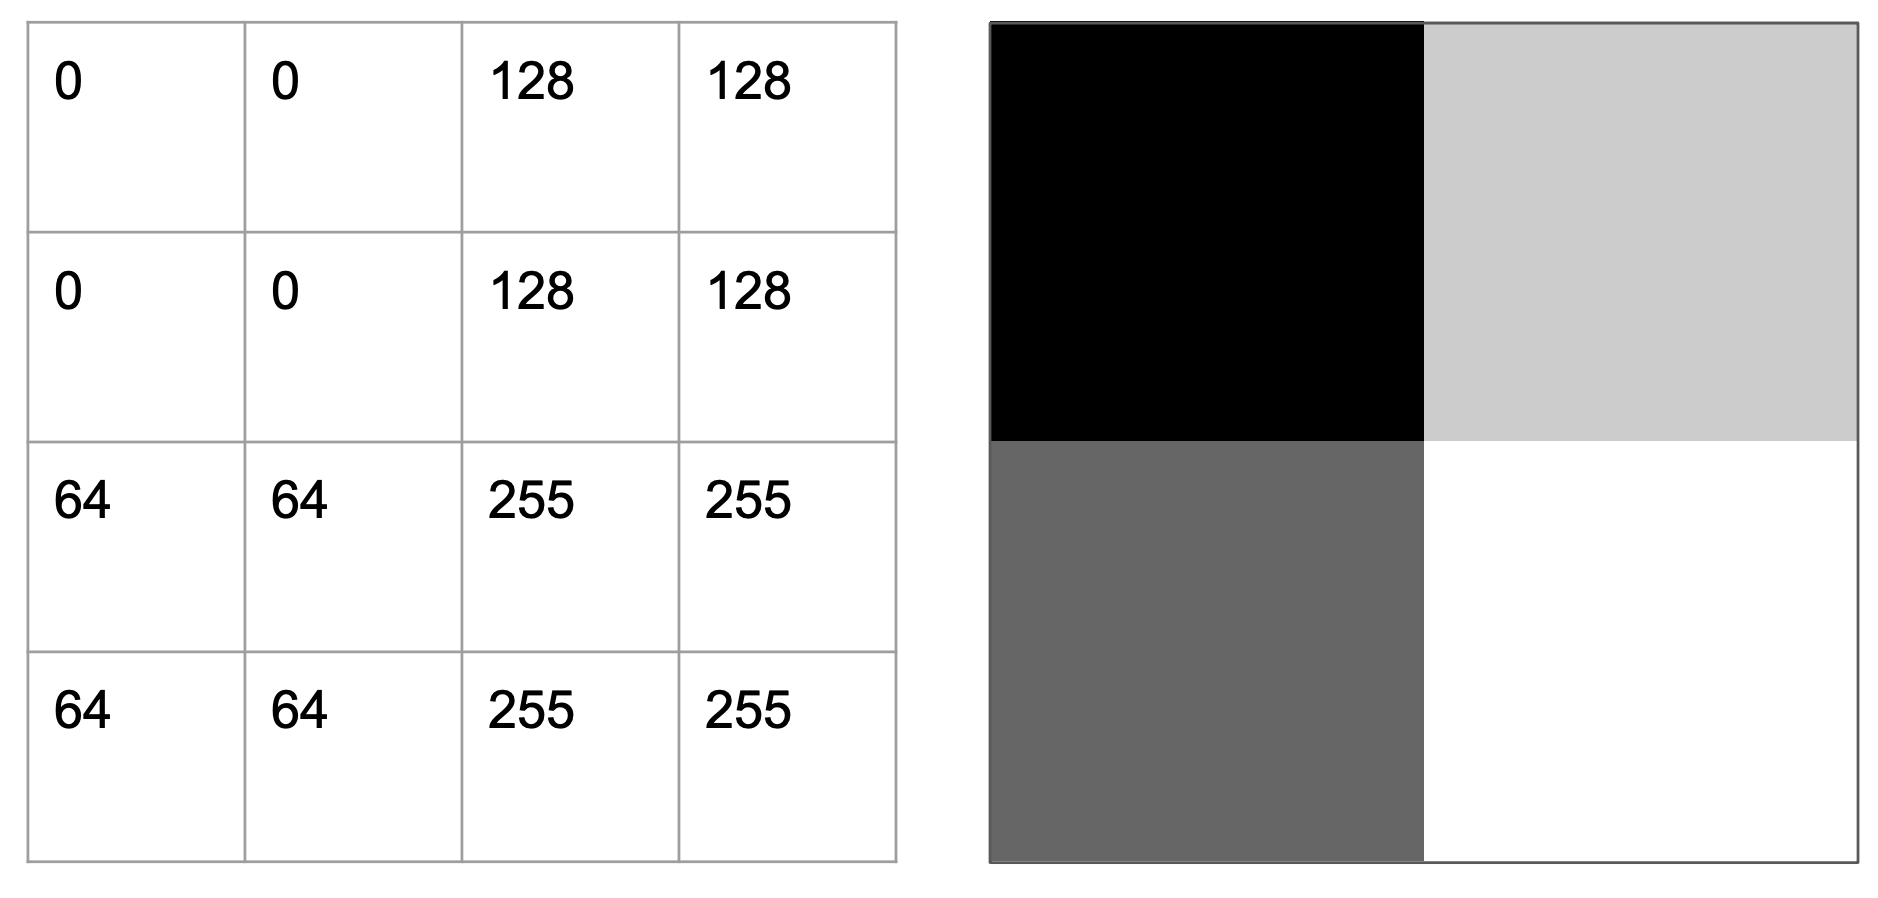
\includegraphics[width=7cm,keepaspectratio]{XX_Figures/Fig_GS.png}
	\caption{\footnotesize Cuatro escalas de grises con su respectivo valor numérico en la matriz izquierda}
	\label{fig:Fig_GS}
\end{figure}

\begin{figure}[p]
	\centering
	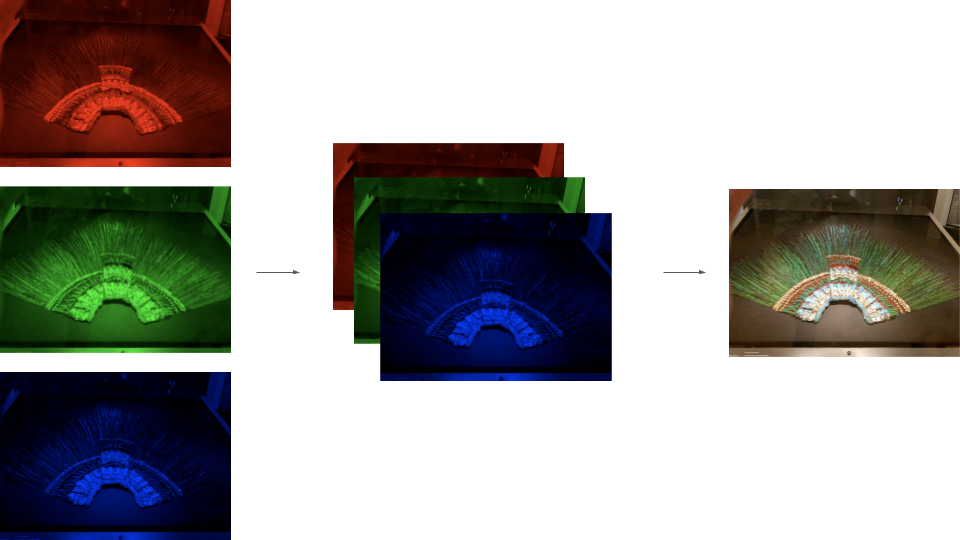
\includegraphics[width=10cm,keepaspectratio]{XX_Figures/Fig_RGB.png}
	\caption{\footnotesize Los tres canales de una imagen en RGB }
	\label{fig:Fig_RGB}
\end{figure}


\begin{figure}[p]
	\centering
	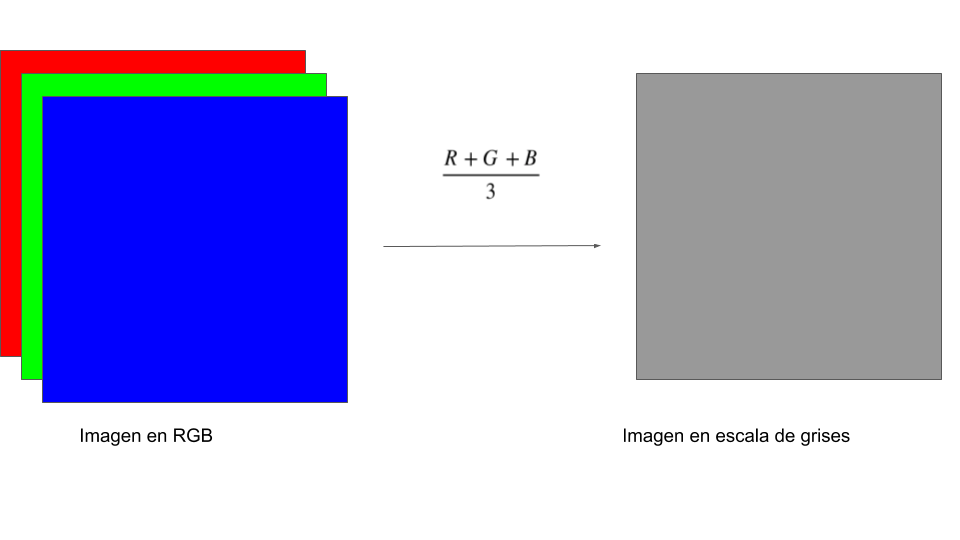
\includegraphics[width=7cm,keepaspectratio]{XX_Figures/Fig_RGBtoGS.png}
	\caption{\footnotesize Conversión de una imagen RGB a escala de grises por promediación}
	\label{fig:Fig_RGBtoGS}
\end{figure}

Una imagen está definida por una función bidimensional \textit{f(x,y)}, donde \textit{x} y \textit{y} son coordenadas espaciales; y la amplitud de \textit{f}  en cualquier par de coordenadas \textit{(x,y)} se llamada intensidad en cualquier punto de la imagen.
Si los valores de \textit{f} son valores finitos discretos, entonces podemos llamar a la imagen una imagen digital. Una imagen digital tiene número finito de elementos y cada uno de estos tiene una localización y valor; a estos elementos se les llaman píxeles \cite{GonzalezDigitalProcessing.pdf}.

Por lo general la mayoría de los píxeles toman valores de 0 a 255 (8 bits); en una imagen en escala de grises 0 representa el  negro y 255 representa blanco, un ejemplo se muestra en la Figura \ref{fig:Fig_GS}.

%----------------------------------------------------------------------------------------
\subsection{RGB}
\label{RGB}

Las imágenes representadas en un modelo RGB, consisten en tres componentes de imágenes como se muestra en la Figura \ref{fig:Fig_RGB}, uno por cada color primario (rojo, verde y azul); cuando estos tres colores alimentan un monitor produce una imagen a color. Considerando que cada uno de los tres canales (R,G,B) contiene 8 bits, al tener una imagen a color tendremos 24 bits de datos, el cuál nos da un posibilidad de tener 16,777,216 colores ($(2^8)^3 = 16,777,216$).\\

----------------------
\subsection{Escala de Grises}
\label{GS}

Una imagen en RGB puede ser convertida a escala de grises (GS) a través de varios métodos. El método más utilizado es por promediación como se muestra en la Figura \ref{fig:Fig_RGBtoGS} en el que los tres valores de los píxeles de los tres planos en la misma posición es sumado y dividido entre tres; esta operación se repite para todos los píxeles para obtener un solo plano.

%----------------------------------------------------------------------------------------
\subsection{Filtros Espaciales}
\label{Filtros_espaciales}

\begin{figure}[th]
	\centering
	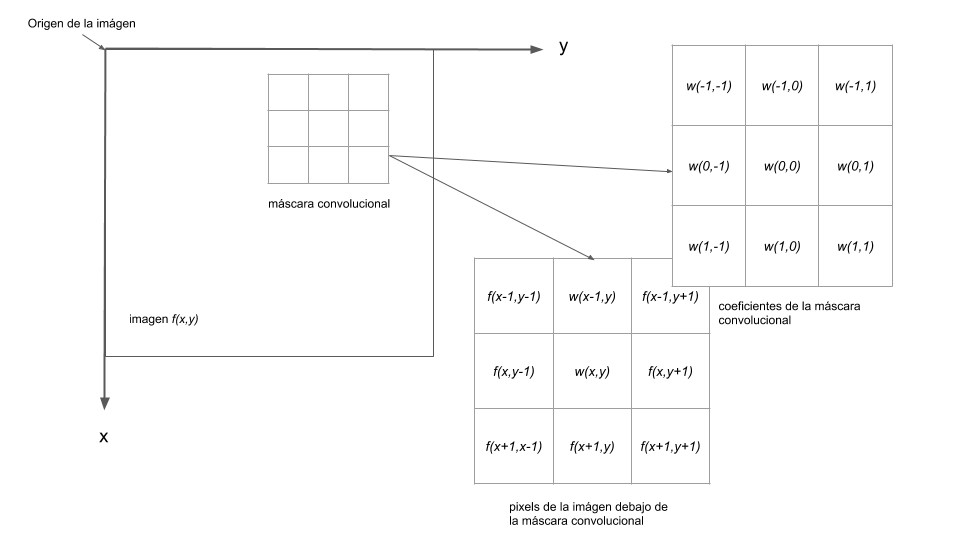
\includegraphics[width=13cm,keepaspectratio]{XX_Figures/Fig4_Convolucion.png}
	\caption{\footnotesize Mecánica del filtraje espacial. El dibujo ampliado muestra una imagen de 3 x 3 y la sección de la imagen que yace directamente bajo ella; la sección de la imagen se muestra desplazada respecto a la máscara para facilitar la legibilidad \cite{GonzalezDigitalProcessing.pdf}}
	\label{fig:Fig4_Convolucion}
\end{figure}

Las operaciones para el filtrado espacial se aplican directamente sobre los píxeles de una imagen como se muestra en la Figura \ref{fig:Fig4_Convolucion}. Para realizar el filtrado  se realiza un barrido de un núcleo (kernel) o máscara de convolución, sobre cada punto de la imagen \cite{GonzalezDigitalProcessing.pdf}. A las máscaras o filtros utilizados, también se le llaman comúnmente como máscaras convolucionales, ya que el proceso del filtrado lineal tiene similitud con el concepto en dominio de la frecuencia llamada convolución. En general, para un filtrado espacial lineal de una imagen \textit{f} de tamaño \textit{M} x \textit{N} con un kernel de tamaño \textit{m} x \textit{n}, la salida de nuestro filtrado está dada por la ecuación \ref{equ:Filtro_lineal}.

\begin{equation}
	\label{equ:Filtro_lineal}
	g(x,y) =  \sum_{s=-a}^{a}\sum_{t=-b}^{b}w(s,t)f(x+s,y+t).\\
\end{equation}

Donde \textit{a = (m-1)/2} y \textit{b = (n-1)/2}, y el filtrado debe ser aplicado para \textit{x = 0,1,2,...,M-1} y \textit{y = 0,1,2,...,N-1}. De esta manera aseguramos que la máscara sea aplicada a todos los píxeles de la imagen. 

Comúnmente para simplificar la notación y no enfocarse en las mecánicas implementadas por una máscara convolucional, solamente en la respuesta obtenida, se utiliza la ecuación \ref{equ:Filtro_lineal_simplicado}.

\begin{equation} 
\label{equ:Filtro_lineal_simplicado}
\begin{split}
R &= w_{1}z_{1} + w_{2}z_{2} + ... + w_{mn}z_{mn} \\
g(x,y) &=  \sum_{i=1}^{mn}w_{i}z_{i}.
\end{split}
\end{equation}

Donde \textit{w's} son los coeficientes de la máscara utilizada y \textit{z's} los valores de una imagen en escala de grises. Esta ecuación es usada más frecuentemente en la literatura de procesamiento de imágenes \cite{GonzalezDigitalProcessing.pdf}.

%-----------------------------------------------------------------------------------------%-----------------------------------------------------------------------------------------
\subsubsection{Sobel}
\label{Sobel}

\begin{figure}[th]
	\centering
	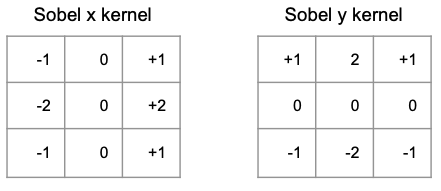
\includegraphics[width=5cm,keepaspectratio]{XX_Figures/Fig_Matrices_Sobel.png}
	\caption{\footnotesize Matrices del operador \textit{Sobel} para detectar bordes.}
	\label{fig:Fig_Matrices_Sobel}
\end{figure}

\begin{figure}[th]
	\centering
	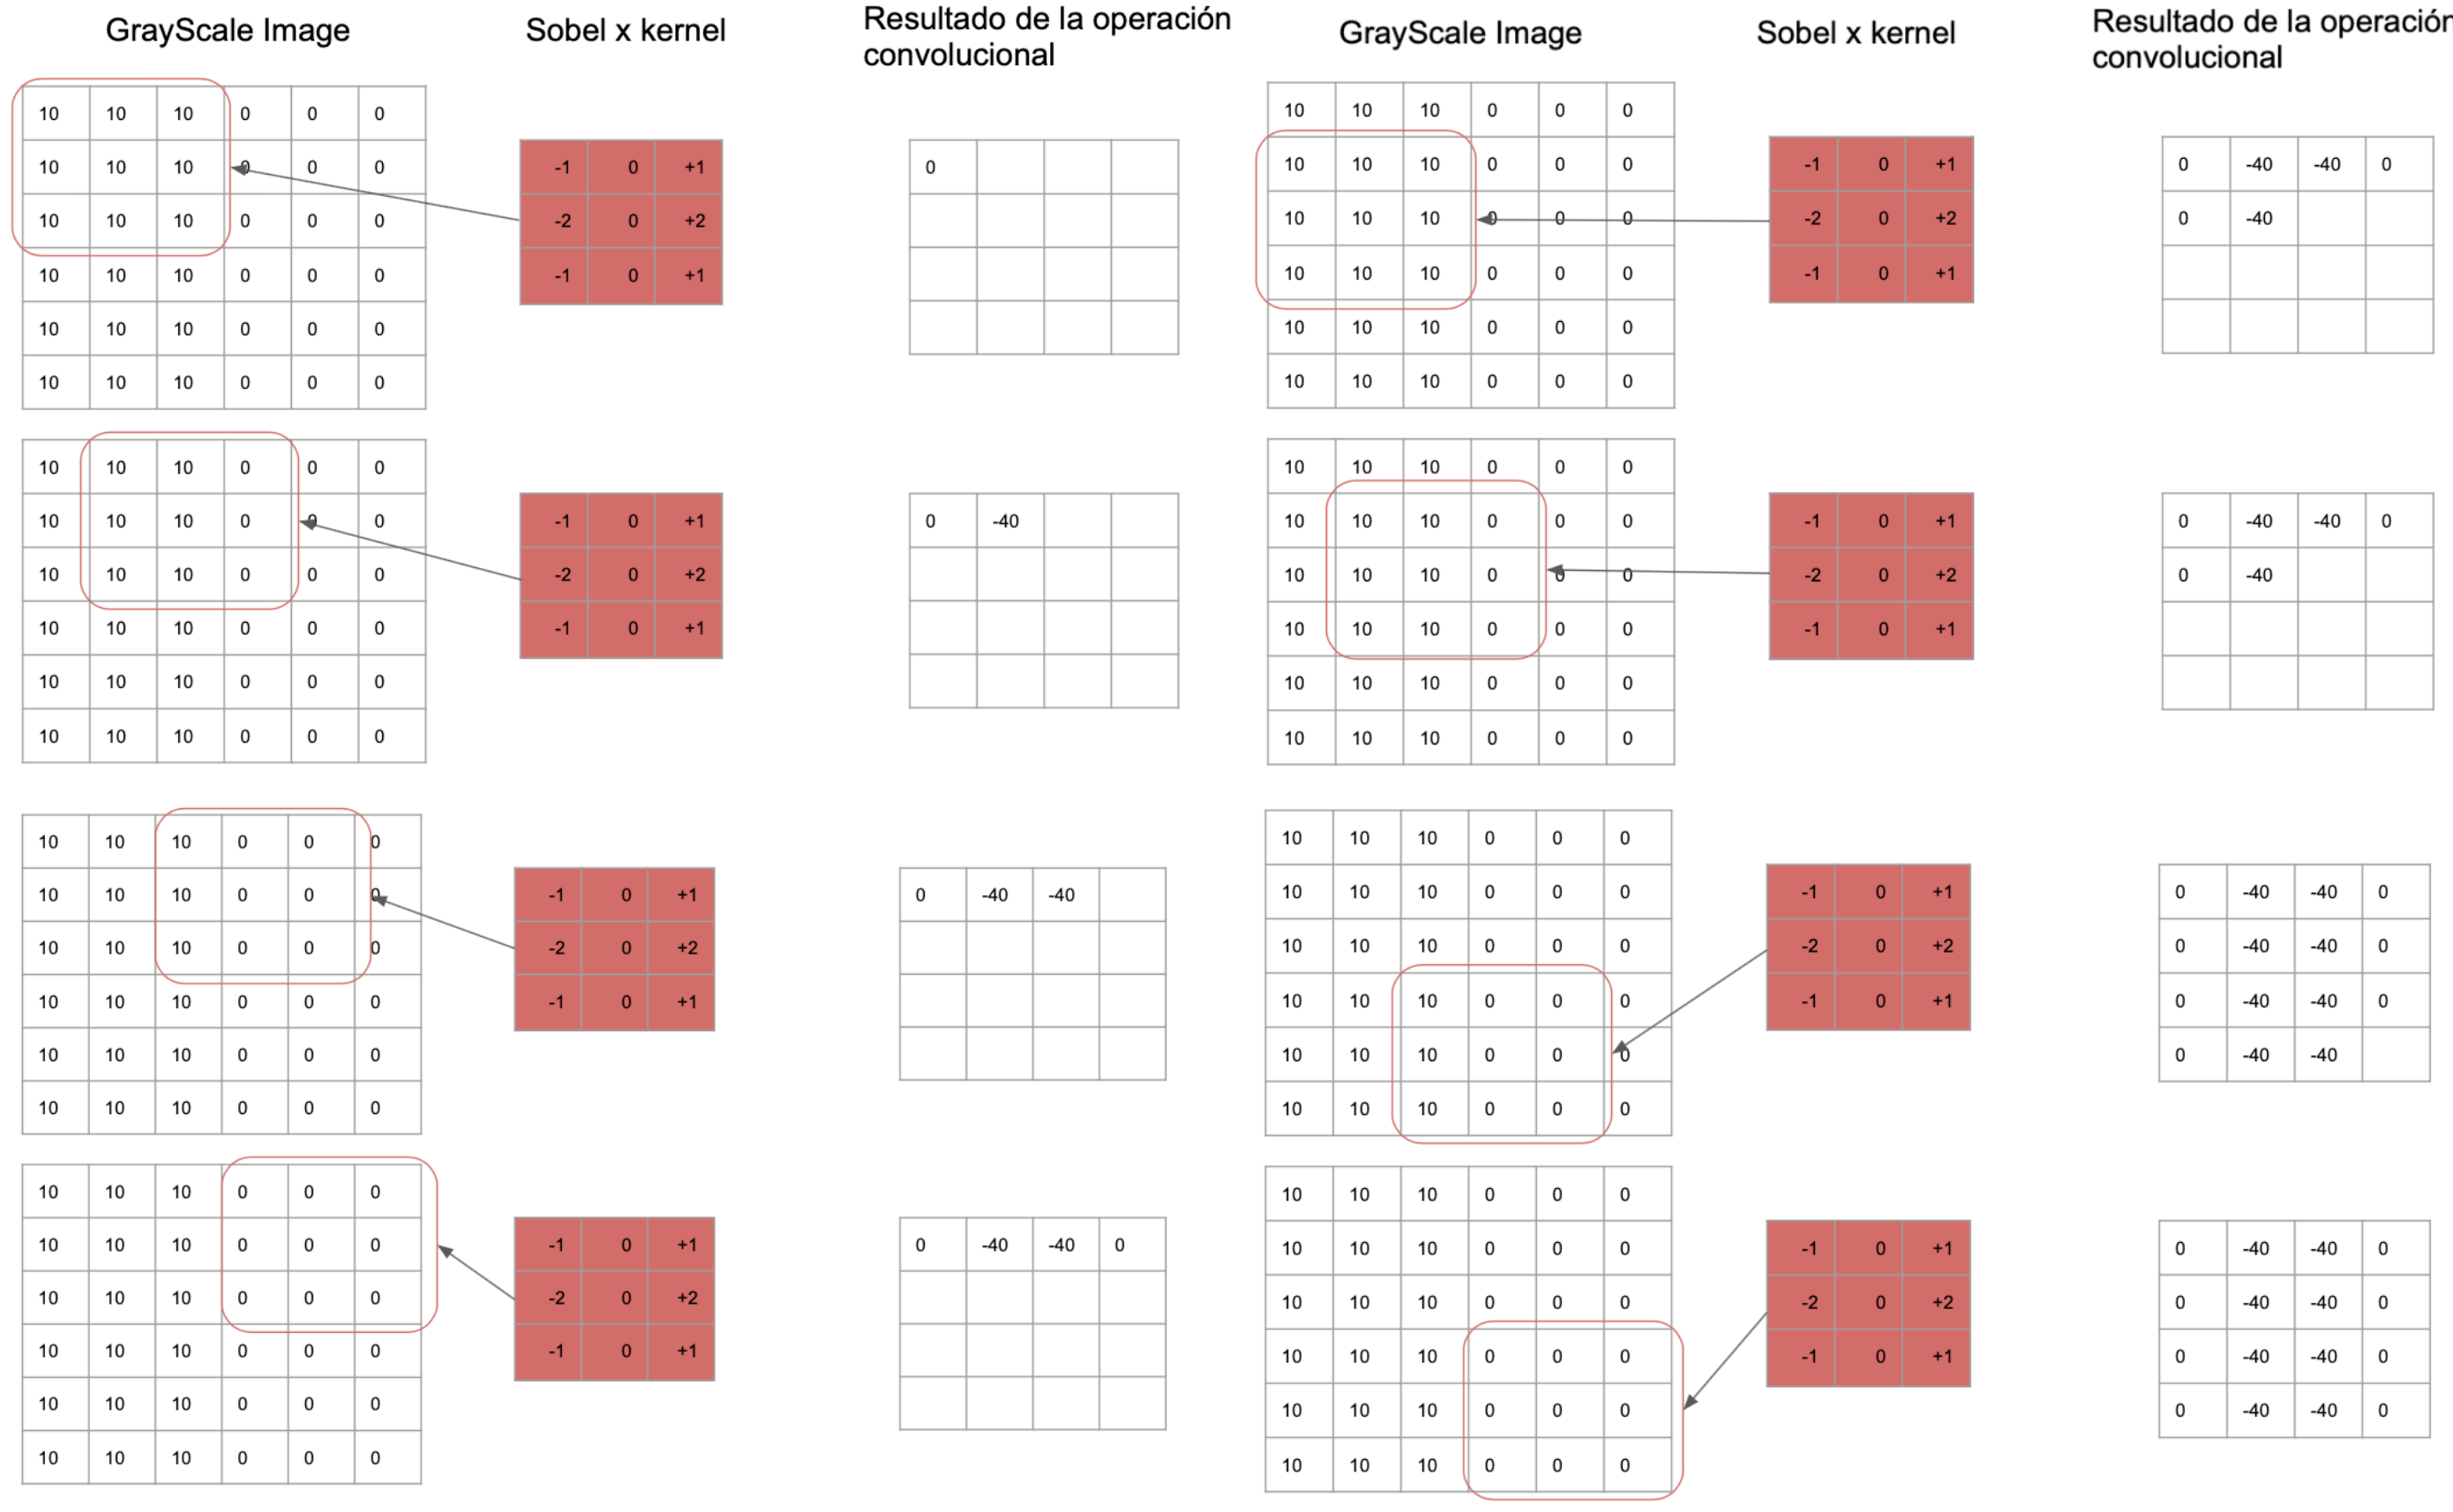
\includegraphics[width=17cm,keepaspectratio]{XX_Figures/Fig_Ejemplo_Sobelx.png}
	\caption{\footnotesize Resultados numéricos al aplicar un filtro \textit{Sobelx} sobre una imagen de 6 x 6}
	\label{fig:Fig_Ejemplo_Sobelx}
\end{figure}

\begin{figure}[th]
	\centering
	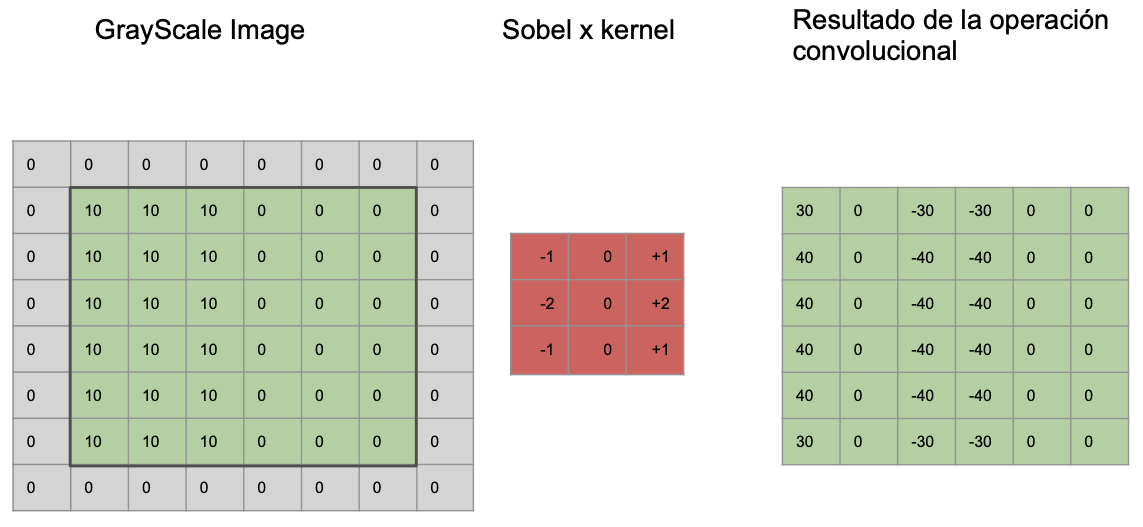
\includegraphics[width=10cm,keepaspectratio]{XX_Figures/Fig_Sobel_padding.png}
	\caption{\footnotesize Relleno de ceros alrededor de los bordes de la imagen}
	\label{fig:Fig_Sobel_padding}
\end{figure}

El operador Sobel es un filtro espacial que tiene como objetivo la detección de los bordes de los objetos en una imagen. Este filtro es utilizado comúnmente para detectar objetos en una imagen a través de los bordes; el operador utiliza un par de matrices de gradiente horizontal y vertical cuyas dimensiones son de 3 x 3 para las operaciones de detección de bordes \cite{Gupta2013SobelAlgorithm}. Estas matrices se muestran en la Figura \ref{fig:Fig_Matrices_Sobel} y en la Figura \ref{fig:Fig_Ejemplo_Sobelx} un ejemplo de cómo se van detectando los bordes utilizando las máscaras convolucionales del operador \textit{Sobely}. Podemos ver que al terminar una operación, el filtro se mueve una posición para seguir con el mismo procedimiento en una localización distinta; a este movimiento se le conoce comúnmente como paso (stride), el cual es el número de desplazamientos de píxeles sobre la matriz de píxeles. En el último paso de la Figura \ref{fig:Fig_Ejemplo_Sobelx} se observa que se obtiene una matriz con valores negativos; esto quiere decir que existe un borde en la imagen y este tiene dirección hacia la izquierda. Si en dado caso se quisiera obtener solamente el filtro \textit{Sobelx} sin dirección, simplemente se obtiene el valor absoluto de todos los píxeles.
Nótese que al aplicar el operador \textit{Sobel} se reduce el tamaño de la imagen resultante. Para evitar este problema, se agrega un relleno (padding) en los bordes de la imagen como se muestra en la Figura \ref{fig:Fig_Sobel_padding}, para que al momento de aplicar nuestro operador y de hacer el barrido por toda la imagen, se obtenga la misma cantidad de píxeles \cite{LaplacianEdgeFilter}. Este relleno es aplicado en varios filtros convolucionales para obtener la misma cantidad de píxeles en los resultados.


%-----------------------------------------------------------------------------------------
\subsubsection{Laplaciano}
\label{Laplaciano}

\begin{figure}[th]
	\centering
	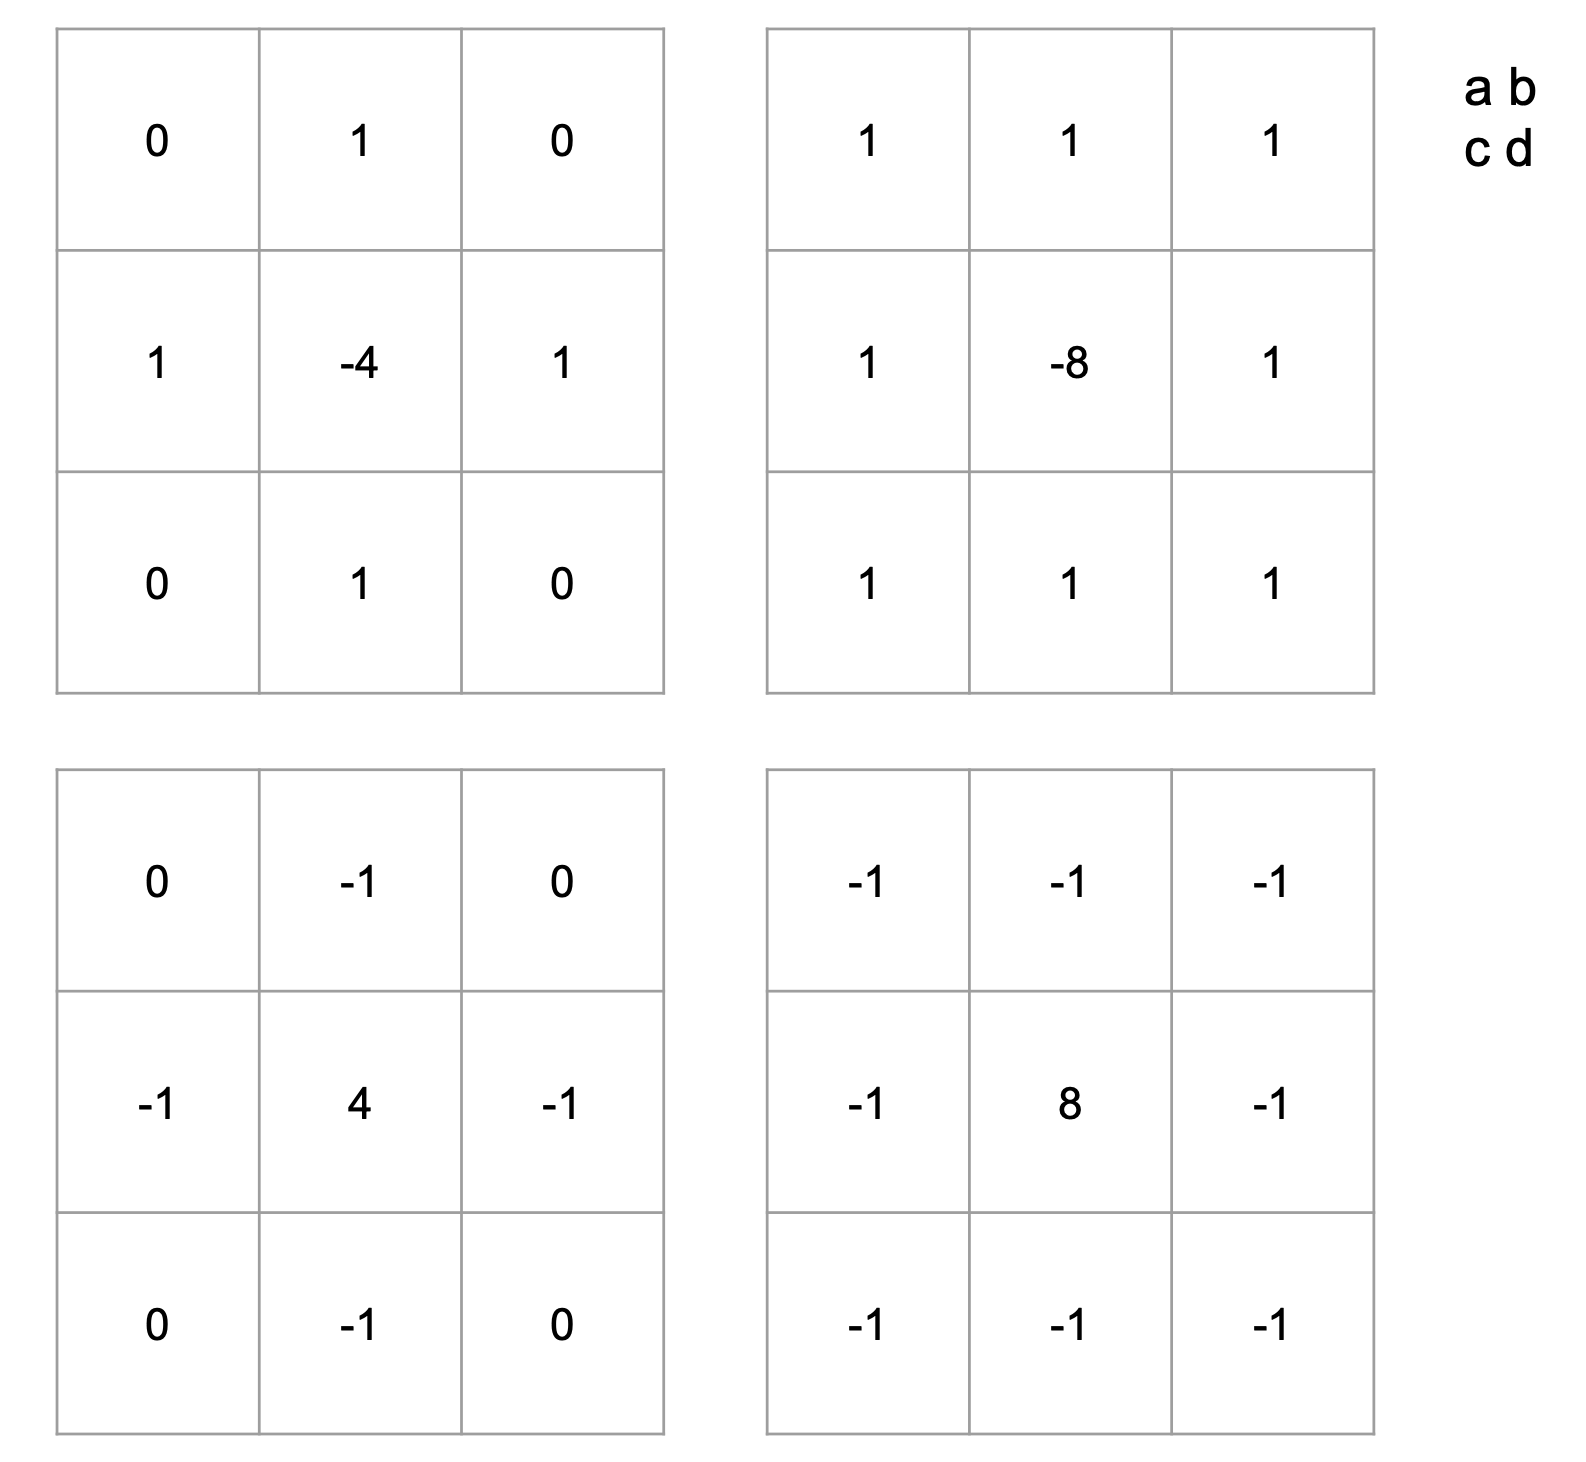
\includegraphics[width=5cm,keepaspectratio]{XX_Figures/Fig_Filtros_Laplacianos.png}
	\caption{\footnotesize Filtros Laplacianos con diferentes cualidades e implementaciones.}
	\label{fig:fig_filtros_laplacianos}
\end{figure}

El filtro Laplaciano es uno de los filtros utilizados con el objetivo de agudizar una imagen y así resaltar detalles que no se lograban ver, posiblemente porque la imagen estaba borrosa.

En la Figura \ref{fig:fig_filtros_laplacianos} podemos ver 4 máscaras convolucionales Laplacianos comúnmente utilizados. En la Figura \ref{fig:Fig_Ejemplo_Laplaciano} se puede notar en la imagen del centro el resultado de aplicar un kernel Laplaciano sobre una imagen y en la imagen de la derecha se observa como la imagen se agudiza y se notan más detalles gracias a la suma escalada del filtro Laplaciano y la imagen original.

\begin{figure}[th]
	\centering
	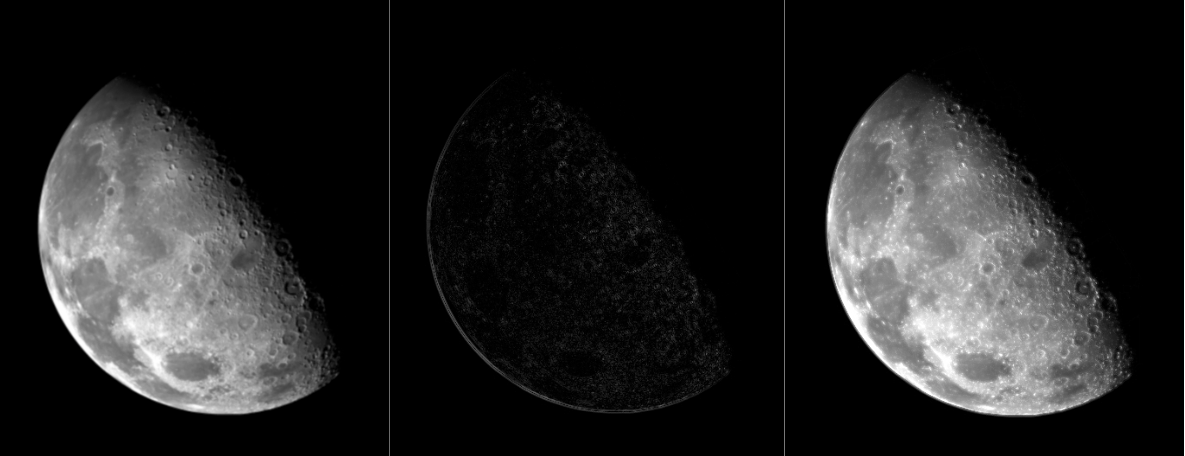
\includegraphics[width=10cm,keepaspectratio]{XX_Figures/Fig_Ejemplo_Laplaciano.png}
	\caption{\footnotesize A la izquierda una imagen de la Luna, al centro el resultado de aplicarle el filtro Laplaciano c de la Figura \ref{fig:fig_filtros_laplacianos} y a su derecha la suma escalada de las dos imágenes previamente mencionadas.}
	\label{fig:Fig_Ejemplo_Laplaciano}
\end{figure}

%----------------------------------------------------------------------------------------
%-----------------------------------------------------------------------------------------
\subsubsection{Kirsch}
\label{Kirsch}

\begin{figure}[th]
	\centering
	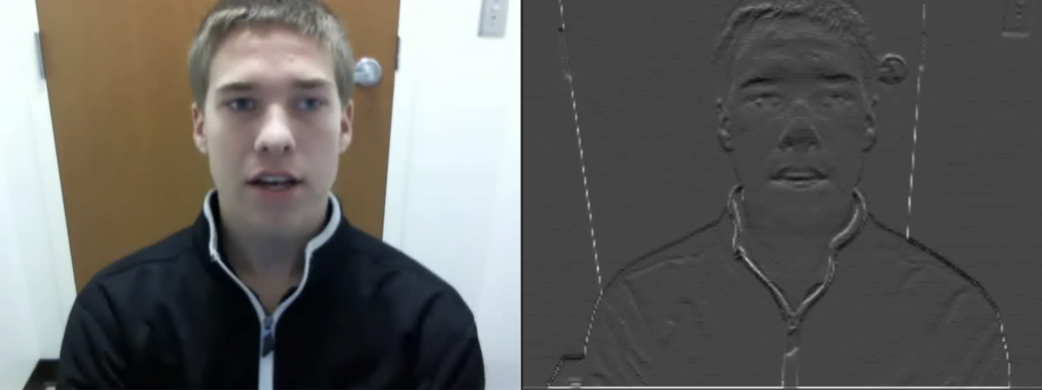
\includegraphics[width=11cm,keepaspectratio]{XX_Figures/Fig_Ejemplo_Kirsch.png}
	\caption{\footnotesize Aplicación del filtro Kirsch.}
	\label{fig:Fig_Ejemplo_Kirsch}
\end{figure}

El filtro Kirsch es un operador detector de bordes que encuentra el borde más significativo en ocho direcciones predeterminadas. La magnitud del borde se obtiene explorando el valor de los píxeles alrededor de ese píxel. Si todos los píxeles en el vecindario tienen casi el mismo valor, entonces probablemente no haya un borde en ese punto. Sin embargo, si algunos de los píxeles alrededor tienen valores mayores que los demás entonces, existe la probabilidad de que haya un borde en ese punto \cite{Kalaiselvi2017ModifiedSegmentation}. El algoritmo Kirsch utiliza un kernel de 3 × 3 y  lo rota 45 grados para así obtener 8 direcciones como se muestra a continuación. 
\begin{align*}
E &= \begin{bmatrix}
-3 & -3 & 5 \\
-3 & 0 & 5 \\
-3 & -3 & 5 
\end{bmatrix},
& 
N &= \begin{bmatrix}
5 & 5 & 5 \\
-3 & 0 & -3 \\
-3 & -3 & -3
\end{bmatrix},
& 
W &= \begin{bmatrix}
5 & -3 & -3 \\
5 & 0 & -3 \\
5 & -3 & -3
\end{bmatrix},
&
S &= \begin{bmatrix}
-3 & -3 & -3 \\
-3 & 0 & -3 \\
5 & 5 & 5
\end{bmatrix},
&\\
NE &= \begin{bmatrix}
-3 & 5 & 5 \\
-3 & 0 & 5 \\
-3 & -3 & -3
\end{bmatrix},
&
NW &= \begin{bmatrix}
5 & 5 & -3 \\
5 & 0 & -3 \\
-3 & -3 & -3
\end{bmatrix},
&
SW &= \begin{bmatrix}
-3 & -3 & -3 \\
5 & 0 & -3 \\
5 & 5 & -3
\end{bmatrix},
&
SE &= \begin{bmatrix}
-3 & -3 & -3 \\
-3 & 0 & 5 \\
-3 & 5 & 5
\end{bmatrix},
\end{align*}


\begin{figure}[th]
	\centering
	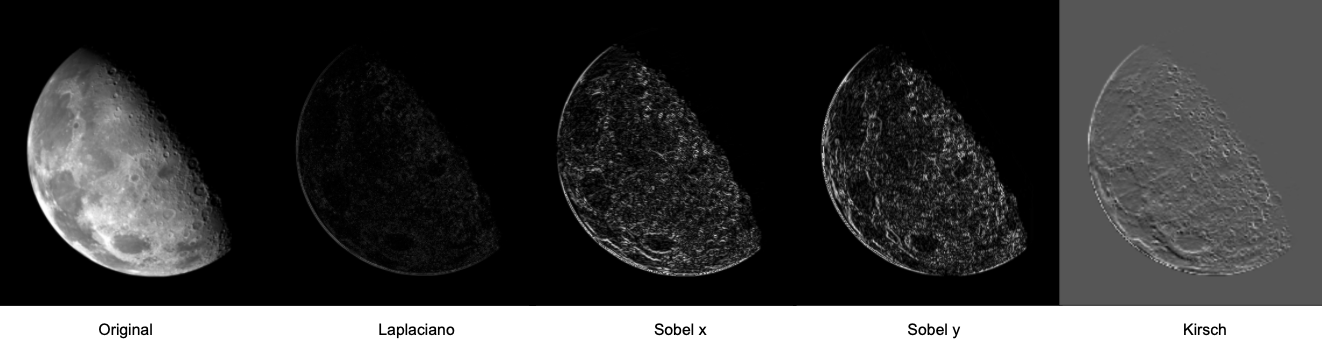
\includegraphics[width=17cm,keepaspectratio]{XX_Figures/Fig_Comparacion_Filtros.png}
	\caption{\footnotesize Comparación de filtros convolucionales para agudización y detección de bordes.}
	\label{fig:Fig_Comparacion_Filtros}
\end{figure}


En la Figura \ref{fig:Fig_Ejemplo_Kirsch}, se puede observar la utilidad de este operador convolucional después de convertir la imagen de RGB a escala de grises y en la Figura \ref{fig:Fig_Comparacion_Filtros} se puede comparar los resultados al aplicar los filtros convolucionales para bordes y agudizamiento mencionados anteriormente. Se debe resaltar que para aplicar todos los filtros mencionados anteriormente, es necesario tener la imagen en escala de grises.\\

Estos filtros son utilizados para resaltar u obtener diferentes características en imágenes, dependiendo de la tarea que se desee realizar.

%-----------------------------------------------------------------------------------------
\subsubsection{Flujo óptico}
\label{OpticalFlow}

El flujo óptico está definido como el movimiento aparente que tiene cada píxel en una imagen. Si se desea analizar el movimiento humano, las expresiones y los gestos, una sola imagen es muy poca información para entender a que clase pertenece un gesto humano. Con el flujo óptico (optical flow) podemos obtener imágenes que representan el movimiento del contexto de la escena en relación con un observador ya que utiliza dos frames que contienen objetos en diferentes posiciones de la imagen y pueden ser utilizados para extraer características temporales.
En la Figura \ref{fig:Fig_OpticalFlow}, se observa un ejemplo del funcionamiento del OpticalFlowX y OpticalFlowY.

\begin{figure}[th]
	\centering
	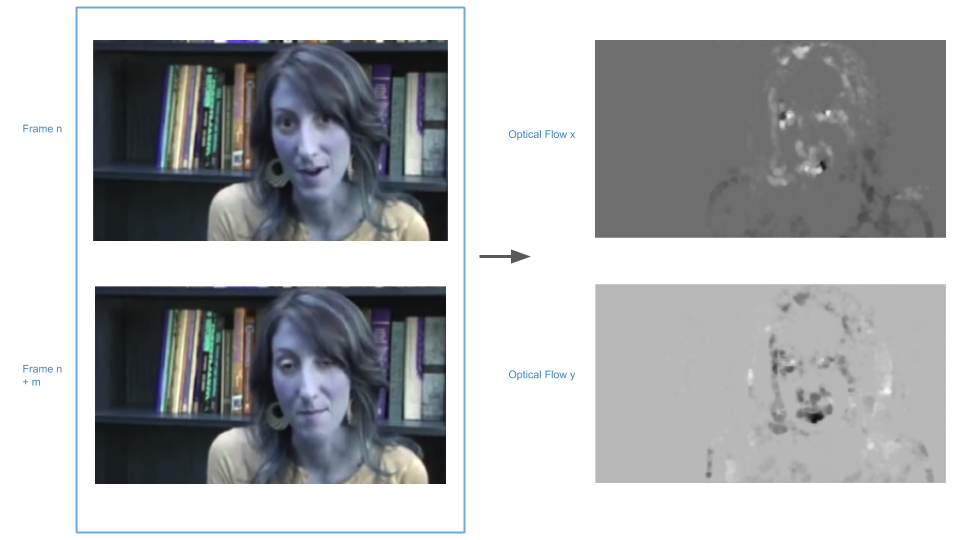
\includegraphics[width=14cm,keepaspectratio]{XX_Figures/Fig_OpticalFlow.png}
	\caption{\footnotesize Flujo óptico de dos imágenes separadas m cantidad de frames.}
	\label{fig:Fig_OpticalFlow}
\end{figure}

%----------------------------------------------------------------------------------------
%----------------------------------------------------------------------------------------
\section{Redes neuronales artificiales}
\label{RNA}
%----------------------------------------------------------------------------------------
Las redes neuronales artificiales (RNA) tratan de emular ciertas características del sistema nervioso, en la cual a través de un estímulo, la neurona brinda una respuesta a ese estímulo. \cite{Chernyatin1968NNDesign} Una red neuronal estándar consiste en conectar procesadores de información llamados neuronas que van produciendo una secuencia de activaciones con un valor real. Las neuronas pueden ser activadas a través de sensores que perciben el ambiente y otras se activan a través de conexiones ponderadas de neuronas previamente activadas. 

Hay tres elementos básicos de un modelo neuronal. El primer elemento es un conjunto de sinapsis, cada una caracterizada con un propio peso o resistencia. A diferencia del peso de una sinapsis cerebral, el peso sináptico de una RNA puede incluir valores reales negativos y positivos. El segundo elemento es un sumador que ayuda a sumar las señales de entrada ponderadas por sus respectivas fuerzas sinápticas de la neurona. El último elemento es una función de activación para limitar la amplitud de la salida de una neurona \cite{Hawkin2014IntriguingFergus}. Varios avances se han logrado al desarrollar programas inteligentes; con las RNAs podemos resolver de manera exitosa problemas como reconocimiento de patrones, predicción, optimización, memorias asociativas y control \cite{Majumder2015ArtificialNetwork}.
	
En años recientes las redes neuronales profundas artificiales (DNN) han mostrado un gran desempeño en reconocimiento de patrones y el aprendizaje máquina. El aprendizaje profundo y no profundo se distinguen por las diferentes profundidades de rutas que generan posibles vínculos de aprendizaje \cite{Schmidhuber2015DeepOverview}. Dependiendo del problema que se esté enfrentando, de cómo están conectadas las neuronas y de las capas que tengamos es cómo se determinará la función y el comportamiento de nuestra arquitectura de red neuronal \cite{Chernyatin1968NNDesign}.
%----------------------------------------------------------------------------------------
\subsection{Perceptrón Multicapa}
\label{MLP}
%----------------------------------------------------------------------------------------
Se ha demostrado que el uso de la perceptrón multicapa (MLP) es una alternativa efectiva para aproximar prácticamente cualquier función uniforme medible ya que a diferencia de otras técnicas convencionales estadísticas, la perceptrón multicapa no realiza suposiciones previas sobre la distribución de los datos. De igual manera puede modelar funciones altamente no lineales y puede ser entrenada para generalizar con precisión cuando se le presentan datos nunca antes vistos \cite{Gardner1998ArtificialSciences}.\\

La MLP consiste en un sistema de neuronas interconectadas como se muestra en la Figura \ref{fig:fig2_MLP}. Cada una de las neuronas están conectadas por pesos y señales de salida las cuales son una función de la suma de las entradas a la neurona modificada por una función de activación. Es la superposición de muchas funciones de transferencia no lineales simples lo que le da a la MLP la capacidad de aproximar funciones no lineales. Si la función de transferencia de la MLP es lineal entonces solo podrá modelar funciones lineales. La salida de las neuronas es escalada por el peso de conexión de la siguiente neurona en la siguiente capa de la red. Una MLP puede llegar a tener una o varias capas ocultas y al final una capa de salida. Las entradas y las salidas de la MLP pueden ser representadas por vectores simples \cite{Gardner1998ArtificialSciences}. \\

\begin{figure}[th]
	\centering
	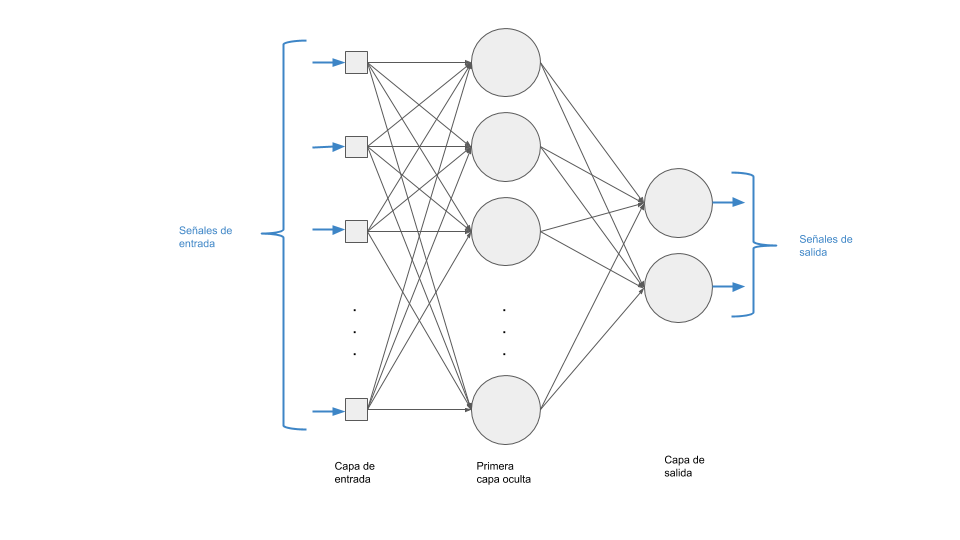
\includegraphics[width=14cm,keepaspectratio]{XX_Figures/fig2_MLP.png}
	\caption{\footnotesize MLP con dos señales de salida.}
	\label{fig:fig2_MLP}
\end{figure}

La MLP tiene la capacidad de aprender a través del entrenamiento, el cual consiste en una serie de entradas asociadas con su vector de salida y los pesos de la red se van ajustando hasta que el mapeo entrada-salida deseado ocurra; para lograrlo es necesario presentarle repetidamente a la red los datos de entrenamiento. Es por esto que la MLP tiene el objetivo de crear una función capaz de predecir el valor correspondiente a una entrada valida después de haber visto una serie de ejemplos en los datos de entrenamiento. Si logramos obtener conjuntos adecuados de pesos y funciones de transferencia, se ha demostrado que la MLP puede aproximarse a cualquier función uniforme y medible entre los vectores de entrada y salida \cite{Caille1980EtudeThymie}. Para lograr que la MLP obtenga pesos y funciones de transferencia que logren la generalización cuando se le presentan datos nunca antes vistos, es necesario entrenarla con datos adecuadamente representativos. Por esta razón el buen funcionamiento de la MLP depende en gran parte de los datos de entrenamiento. 

Por lo general en la etapa de entrenamiento, puede que la salida de la MLP no sea igual a la salida deseada, por lo que se calcula una señal de error definida como la diferencia entre la salida deseada y la salida real; esta señal es usada en el entrenamiento para determinar en qué grado se deben ajustar los pesos en la red y de esta manera el error pueda ser reducido. Por lo anterior, el objetivo del entrenamiento es encontrar la combinación de pesos el cual nos dará el punto mínimo para la superficie del error. 

%El algoritmo de retropropagación (back-propagation algorithm) es el algoritmo más sencillo computacionalmente para entrenar una MLP. Este algoritmo ocupa el procedimiento del gradiente descendiente para tratar de encontrar el mínimo global de la superficie del error y los pasos que sigue se resumen a continuación:%

%\begin{enumerate}
%        \item Inicializar los pesos de la red.
%    \item Presentar el primer vector de entrada del conjunto de entrenamiento a la red.
%    \item Propagar el vector de entrada a través de la red para obtener una salida.
%    \item Calcular la señal de error comparando la salida actual con la salida deseada.
%    \item Propagar la señal de error hacia atrás a través de la red (Figura \ref{fig:fig1_Senal_de_error}).
%    \item Ajustar los pesos para minimizar el error global.
%    \item Repetir los pasos 2-7 con el siguiente vector de entrada, hasta que el error global sea satisfactoriamente pequeño.
%\end{enumerate}

%\begin{figure}[th]
%	\centering
%	\includegraphics[width=11cm,keepaspectratio]{XX_Figures/%fig1_Senal_de_error.png}
%	\caption{\footnotesize Retropropagación de la señal de %error en una MLP.}
%	\label{fig:fig1_Senal_de_error}
%\end{figure}

\begin{figure}[th]
	\centering
	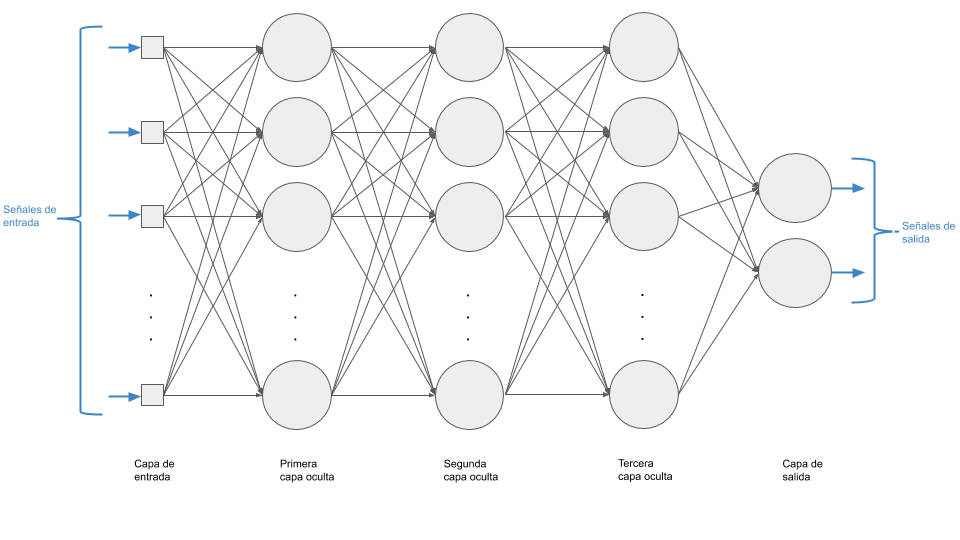
\includegraphics[width=16cm,keepaspectratio]{XX_Figures/fig3_MLP_profunda.png}
	\caption{\footnotesize MLP con tres capas ocultas y dos señales de salida.}
	\label{fig:fig3_MLP_profunda}
\end{figure}

%En este algoritmo los pesos de la red se adaptan después de que cada patrón ha sido presentado y a este método  se le conoce como on-line training; es un método en el cual la los datos se presentan de manera secuencial y es usado para actualizar nuestro modelo para futuros datos. Esta manera de entrenar es comúnmente utilizada para adaptar dinámicamente nuestro modelo a nuevos patrones o cuando los datos por sí mismos son generados en función del tiempo. Otra alternativa es conocida como batch training en la que la suma de todos los patrones es utilizada para actualizar los pesos de la red. De igual forma es necesario el paso de varias iteraciones de entrenamiento para que la red alcance un error satisfactoriamente bajo. El entrenamiento de la red no necesariamente debe terminar cuando se haya alcanzado un error global bajo deseado; también puede finalizar cuando en un conjunto de pruebas independiente, se haya alcanzado un desempeño satisfactorio.%
	
%El algoritmo de retropropagación contiene dos parámetros; uno es la tasa de aprendizaje (learning rate) el cuál controla qué tanto se debe cambiar el modelo en respuesta al error estimado cada vez que los pesos de la red es actualizado. Si el learning rate es muy pequeño entonces puede que el entrenamiento tome bastante tiempo en finalizar, en cambio si es muy grande entonces puede que el error de la red cambie erráticamente debido a grandes cambios en los pesos, resultando en la posibilidad de saltar sobre el error mínimo global. El segundo parámetro es el momentum el cual ayuda a acelerar el entrenamiento ya que en dado caso de que quedemos atrapados en un mínimo local y eso nos haga pensar de que hemos alcanzado un mínimo global, el  momentum toma un valor del 0 al 1, si es 1 o cercano, acelera el tamaño de los pasos tomados para poder salir de un mínimo local.%

\subsection{Perceptrón Multicapa Profunda}
\label{MLP_Profunda}

Si la cantidad de capas ocultas es mayor a tres (incluyendo capa de entrada y capa de salida), nuestra MLP califica como una perceptrón multicapa profunda (deep MLP) como se muestra en la Figura \ref{fig:fig3_MLP_profunda}, ya que cada capa contiene características de las señales de entrada con diferente nivel de abstracción; esto sucede porque cada capa de neuronas se entrena en un conjunto distinto de características basadas en la salida de la capa  anterior. Por esta razón, cuando más capas ocultas se tengan, más complejas serán las características que las neuronas pueden reconocer, ya que agregan y combinan características de las capas anteriores. Estrictamente se puede definir como una perceptrón multicapa profunda cuando se tiene más de una capa oculta.
	

%----------------------------------------------------------------------------------------
\subsection{Redes Neuronales Convolucionales}
\label{CNN}
%----------------------------------------------------------------------------------------
Este tipo de arquitectura de red neuronal profunda está inspirado por el mecanismo de percepción visual de los mamíferos y la principal razón es porque la corteza visual de los mamíferos consiste en conjunto de capas con células simples y células complejas; a medida que una imagen es procesada por la corteza visual, se detectan características progresivamente más ricas de la imagen. Las redes neuronales convolucionales (CNNs) consisten de conjuntos de capas convolucionales (convolutional layers) las cuáles se asimilan a las células simples, y conjuntos de capas de agrupación (pooling layers) que asimilan a las células complejas. Se ha demostrado que las CNNs aprenden progresivamente características de nivel superior en forma de filtros en las capas convolucionales \cite{Lecun2015DeepLearning}.\\

Las CNNs son particularmente adecuadas para manejar datos con un cierta estructura de información, tales como señales en audio en la cual la estructura está en una dimensión (vector simple), imágenes en dos dimensiones (una matriz de píxeles) y videos en tres dimensiones (varias matrices de píxeles). La estructura con la cual vamos a manejar los datos puede ayudar a mejorar el desempeño de nuestro modelo. En el caso de las MLPs con el objetivo de aprender a través de los datos de entrenamiento, nos vemos forzados convertir la estructura de nuestros datos (ej. Una matriz) a un vector simple.\\

\begin{figure}[th]
	\centering
	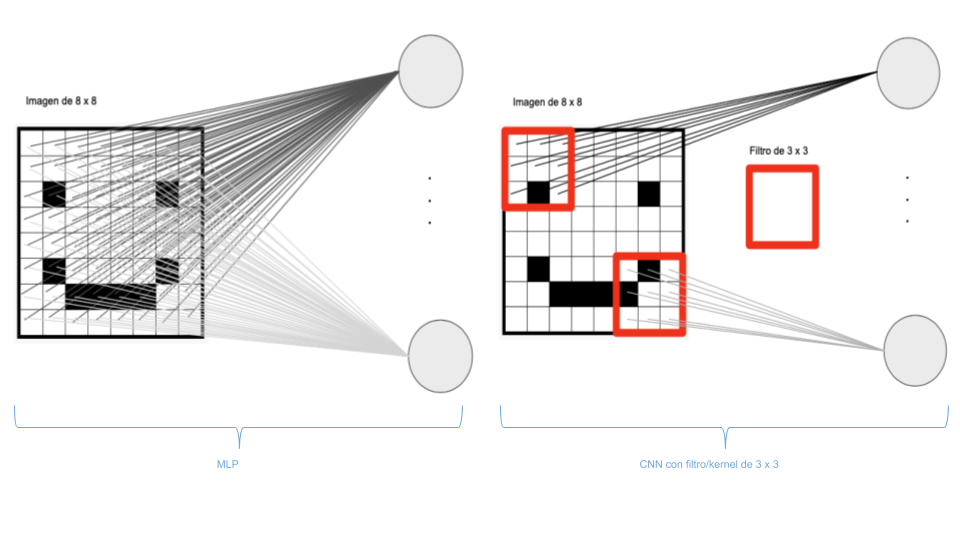
\includegraphics[width=13cm,keepaspectratio]{XX_Figures/Fig_Comparacion_MLP_CNN.png}
	\caption{\footnotesize Comparación de la conectividad de las neuronas entre una MLP y una CNN}
	\label{fig:Fig_Comparacion_MLP_CNN}
\end{figure}

Al igual que la MLP mencionada en el capítulo \ref{MLP}, las redes neuronales convolucionales, están conformadas de neuronas con pesos entrenables y biases. Cada neurona recibe varias entradas y se repite el mismo procedimiento; pero a comparación con la MLP en la que todas las neuronas de alguna capa \textit{n} están completamente interconectadas con la capa \textit{n-1} (Figura \ref{fig:fig3_MLP_profunda}), a cada neurona de la CNN se le conectan algunas neuronas cercanas de la capa anterior como se muestra en la Figura \ref{fig:Fig_Comparacion_MLP_CNN} y un mismo grupo de pesos es utilizado para cada neurona de salida, reduciendo considerablemente la cantidad de operaciones que se necesitan como se muestra en la Figura \ref{fig:Fig_Compartiendo_pesos} ya que las neuronas comparten parámetros y por lo tanto se requieren menos requerimientos computacionales.\\

\begin{figure}[th]
	\centering
	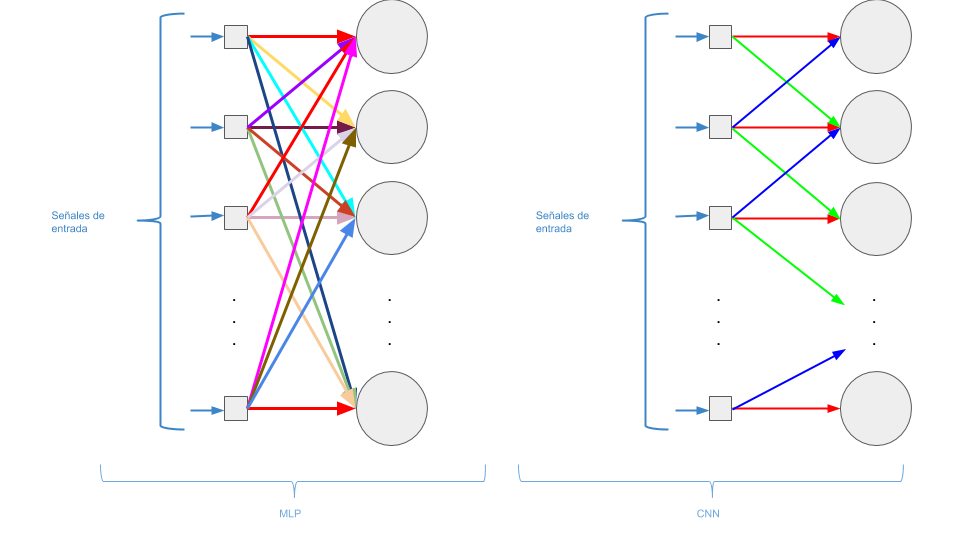
\includegraphics[width=14cm,keepaspectratio]{XX_Figures/Fig_Compartiendo_pesos.png}
	\caption{\footnotesize Comparación de pesos entre una MLP y una CNN.}
	\label{fig:Fig_Compartiendo_pesos}
\end{figure}

%En el siguiente ejemplo se puede notar claramente la reducción de parametros utilizados entre una CNN y una MLP:
%Si nostros tenemos una imagen en RGB de 224 x 224 \textit{pixeles} , entonces tendremos como entrada \textit{x = 224*224*3}, y deseamos tener en la siguiente capa 224,224\\


Este patrón de conexión tiene sentido cuando se pueden extraer características de los datos de manera espacial tal y como funciona una convolución explicado en el Capítulo \ref{Filtros_espaciales}, en la cual se ocupaban las operaciones convolucionales para extraer características de imágenes digitales como resaltar los bordes de los objetos, agudizar la imagen, etc. De igual forma las operaciones convolucionales en las CNNs tienen los mismos atributos mencionados anteriormente en el Capítulo \ref{Filtros_espaciales}, tales como el relleno (Padding) y los pasos (Strides).\\

\subsubsection{2D CNN}
\label{2DCNN}

Por lo general la mayoría de las imágenes se encuentran en escala de grises (GS) o a color; si las imágenes se encuentran en RGB entonces tenemos 3 matrices, cada matriz representa un plano de color como se muestra en el Capítulo \ref{RGB}, por lo tanto, la operación convolucional es aplicada para más de una matriz de características. Para lograr esta operación es necesario agregar profundidad a nuestro filtro convolucional, dependiendo de cuántos canales o mapas de características se tengan como entrada. De igual forma se puede aplicar diferentes filtros convolucionales a un mismo mapa de características de entrada, con la finalidad de extraer más características por capa convolucional.\\

\begin{figure}[th]
	\centering
	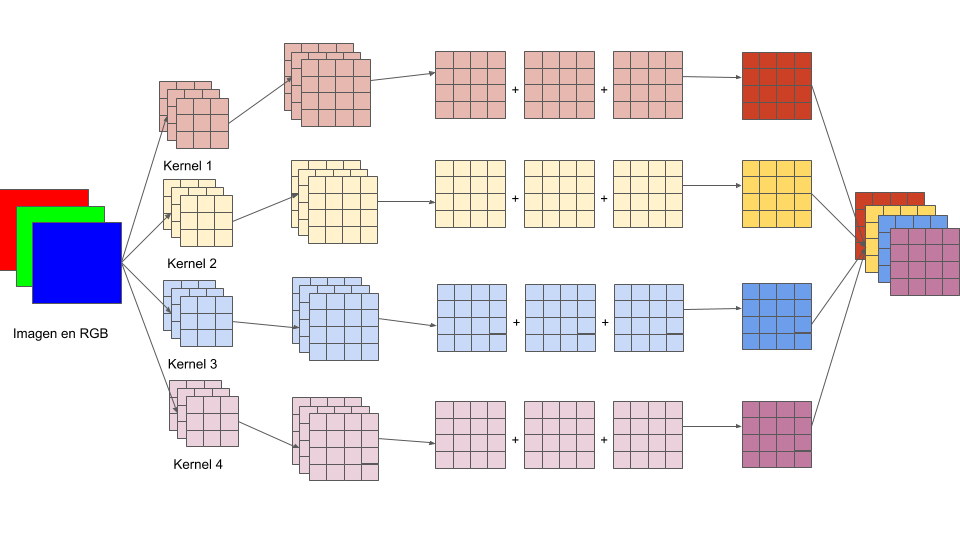
\includegraphics[width=16cm,keepaspectratio]{XX_Figures/Fig_Mapa_caracteristicas.png}
	\caption{\footnotesize Aplicación de filtros convolucionales 2D para obtener mapas de características}
	\label{fig:Fig_Mapa_caracteristicas}
\end{figure}

En la Figura \ref{fig:Fig_Mapa_caracteristicas} se puede observar un ejemplo de cómo se aplican los filtros convolucionales 2D con profundidad de canales. En el ejemplo se aplica una capa convolucional de 4 filtros; cada filtro tiene la misma profundidad que los mapas de características de entrada (imagen en RGB), cada filtro convolucional se aplica por separado para cada canal para así obtener en total 12 mapas de características (3 mapas por filtro convolucional), luego se suman los mapas de características obtenidos por los filtros y se obtiene un mapa de características por cada uno de los 4 kernels. El resultado (4 mapas de características) es nuestro conjunto de mapas de características obtenido al aplicar los cuatro filtros convolucionales.\\

\begin{figure}[th]
	\centering
	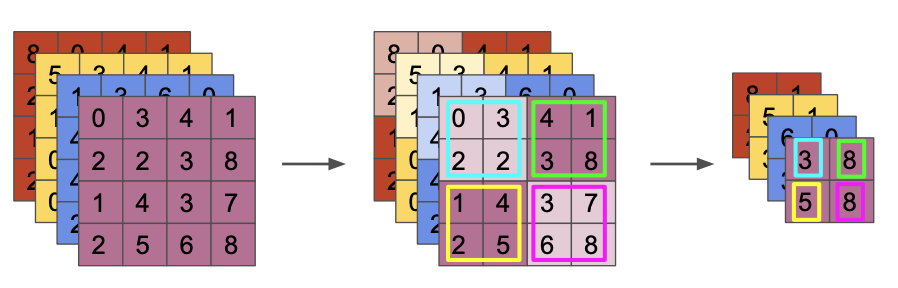
\includegraphics[width=14cm,keepaspectratio]{XX_Figures/Fig_Maxpooling.png}
	\caption{\footnotesize Aplicación de maxpooling de 2 x 2 a la salida mostrada en la Figura \ref{fig:Fig_Mapa_caracteristicas}}
	\label{fig:Fig_Maxpooling}
\end{figure}

La otra operación importante de las CNNs es la agrupación, (pooling) que asimila la labor que tienen las células complejas de la corteza visual de los mamíferos como se mencionó anteriormente. Las capas de agrupación (pooling layers) reducen la cantidad de parámetros que se tienen; esto se logra reduciendo dimensionalmente cada mapa de características obtenidos por nuestra capa convolucional. Hay diferentes capas de agrupación, pero la más usada es la MaxPooling Layer. Esta toma el elemento mas significativo de una ventana definida de nuestro mapa de características.\\

En la Figura \ref{fig:Fig_Maxpooling}, se observa la continuación del ejemplo de la Figura \ref{fig:Fig_Mapa_caracteristicas}, se le añadieron valores numéricos para poder explicar el funcionamiento de la operación maxpooling. Después de aplicar los 4 kernel convolucionales y obtener 4 mapas de características, se aplica un maxpooling de 2 x 2. El mapa de características delantero (morado), es dividido en ventanas de 2 x 2 y para cada una de las ventanas se obtiene el valor más grande. Esta operación se realiza para cada mapa de características. De esta manera se logra reducir el número de parámetros y obtener el valor más significativo de cada ventana en la que fueron divididos los mapas de características.

\begin{figure}[th]
	\centering
	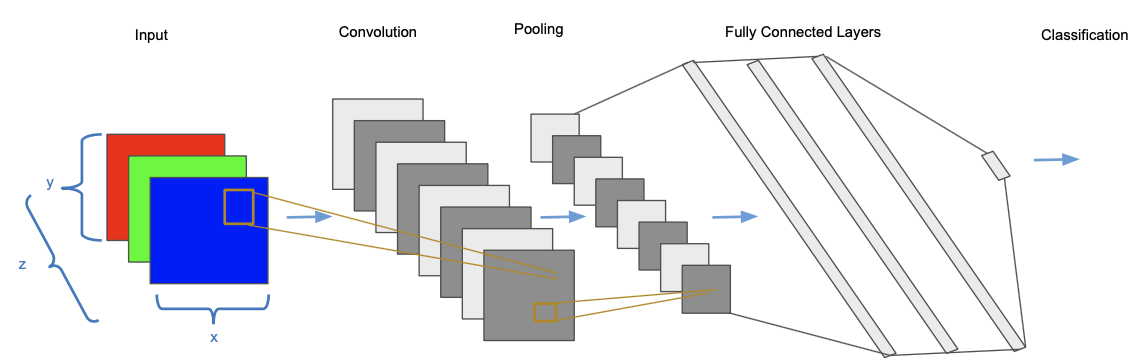
\includegraphics[width=16cm,keepaspectratio]{XX_Figures/Fig_CNN_Arquitecture.png}
	\caption{\footnotesize Arquitectura general de una CNN con una MLP profunda}
	\label{fig:Fig_CNN_Arquitecture}
\end{figure}

\begin{figure}[th]
	\centering
	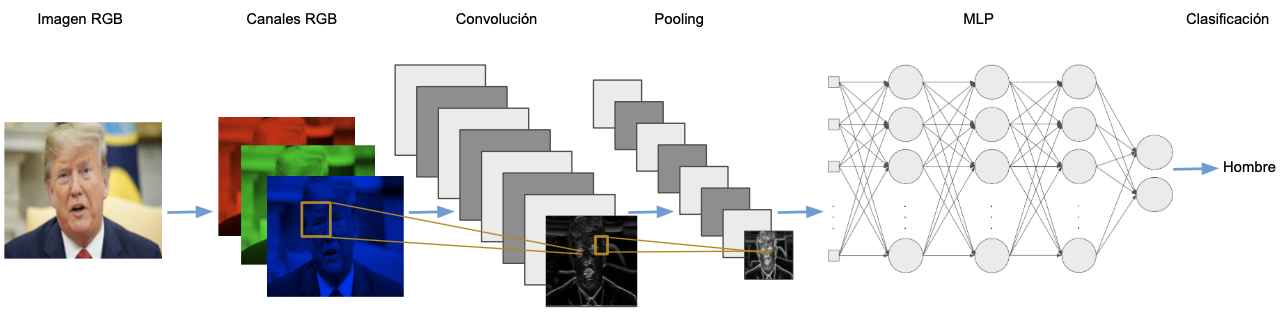
\includegraphics[width=17cm,keepaspectratio]{XX_Figures/Fig_CNN_Example.png}
	\caption{\footnotesize Ejemplo de la aplicación de una CNN con una MLP profunda}
	\label{fig:Fig_CNN_Example}
\end{figure}

Las CNNs son comúnmente utilizadas para extraer características en imágenes de una manera más práctica a comparación con las MLPs ya que requieren menos parámetros para la extracción automática de características en señales, imágenes o video. En la Figura \ref{fig:Fig_CNN_Arquitecture}, se muestra un esquema de cómo se utilizan las CNNs; se observa que una vez finalizada la extracción de características, se utiliza la salida de las CNNs como la entrada de la MLP encargada de igual forma de la extracción de más características y de la tarea de clasificación que se desea, como se muestra en el ejemplo de la Figura \ref{fig:Fig_CNN_Example}.

%----------------------------------------------------------------------------------------
\subsubsection{3D CNN}
\label{3DCNN}
%----------------------------------------------------------------------------------------

Este tipo de arquitectura de red convolucional se aplica cuando se requieren obtener características espaciales (como en la Figura \ref{fig:Fig_CNN_Example}) y características temporales.\\

\begin{figure}[p]
	\centering
	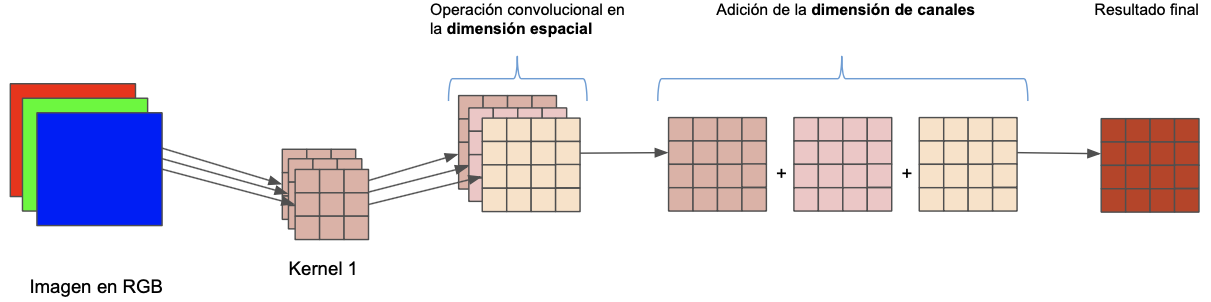
\includegraphics[width=13cm,keepaspectratio]{XX_Figures/Fig_2D_Dimensiones.png}
	\caption{\footnotesize Dimensiones y operaciones de una 2D CNN con un kernel}
	\label{fig:Fig_2D_Dimensiones}
\end{figure}

\begin{figure}[p]
	\centering
	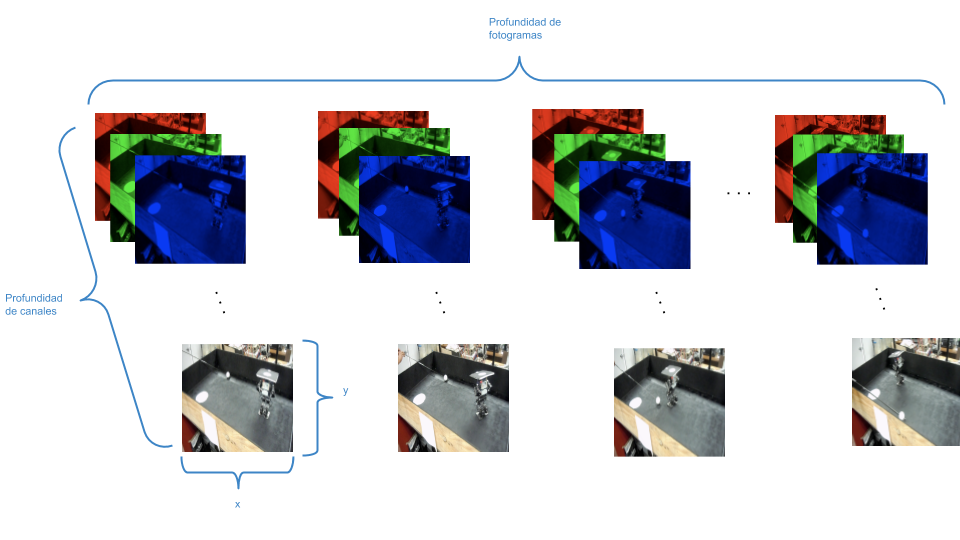
\includegraphics[width=13cm,keepaspectratio]{XX_Figures/Fig_Video.png}
	\caption{\footnotesize Las 4 dimensiones que posee un video}
	\label{fig:Fig_Video}
\end{figure}

\begin{figure}[p]
	\centering
	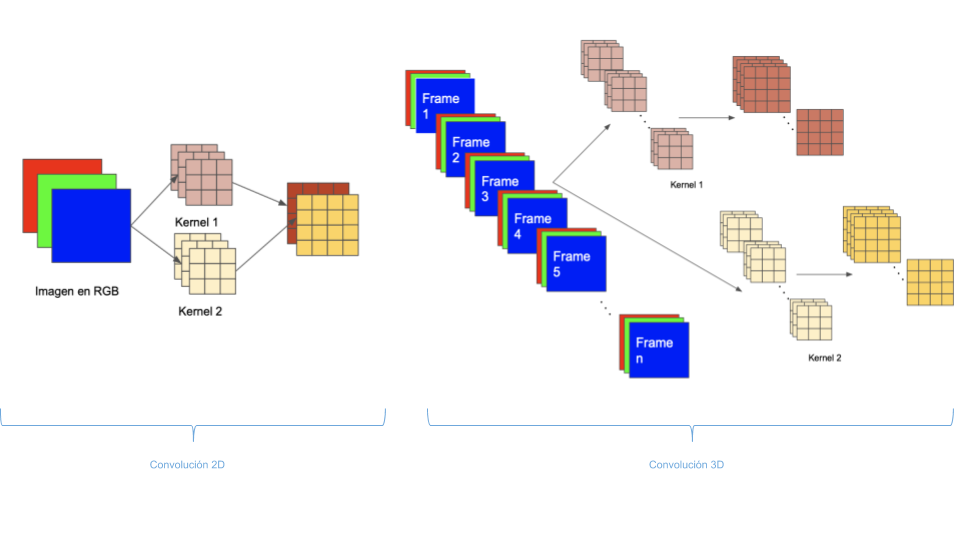
\includegraphics[width=13cm,keepaspectratio]{XX_Figures/Fig_CNN_2Dvs3D.png}
	\caption{\footnotesize Diferencias entre una convolución 2D y 3D}
	\label{fig:Fig_CNN_2Dvs3D}
\end{figure}

\begin{figure}[p]
	\centering
	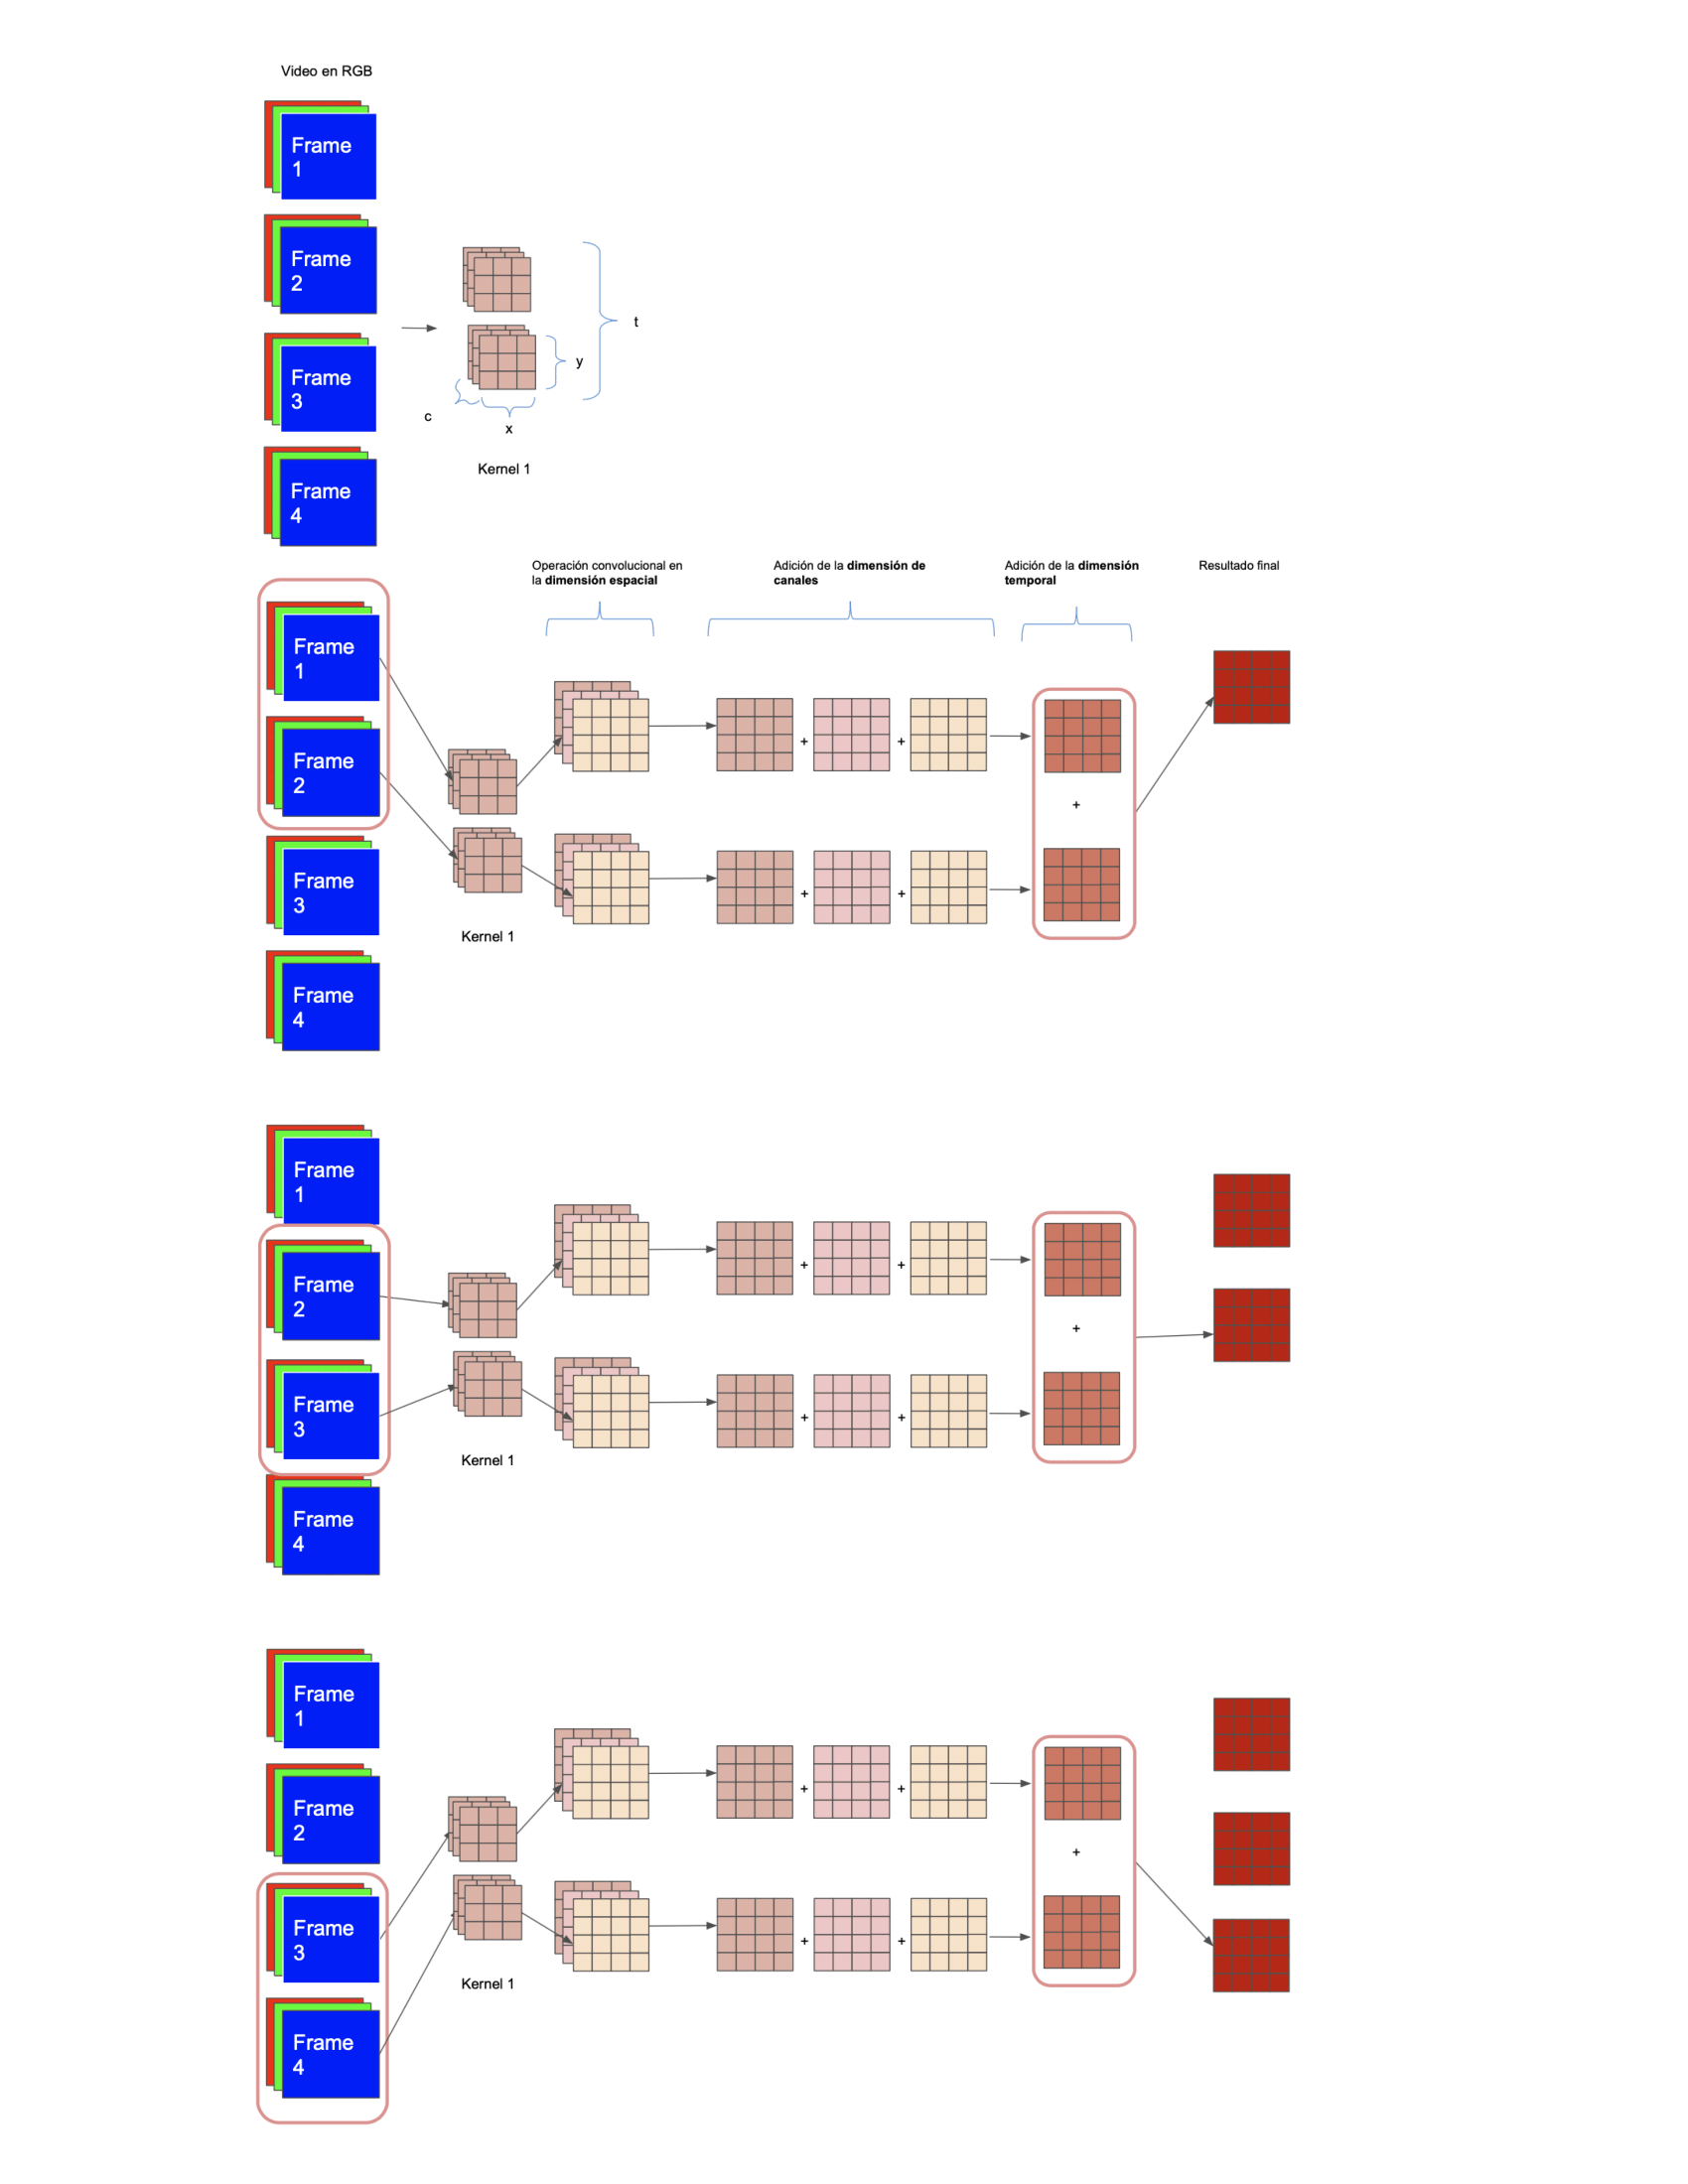
\includegraphics[width=18cm,keepaspectratio]{XX_Figures/Fig_Ejemplo_3DCNN.png}
	\caption{\footnotesize Ejemplo de los pasos en una 3D CNN con un kernel}
	\label{fig:Fig_Ejemplo_3DCNN}
\end{figure}

\begin{figure}[p]
	\centering
	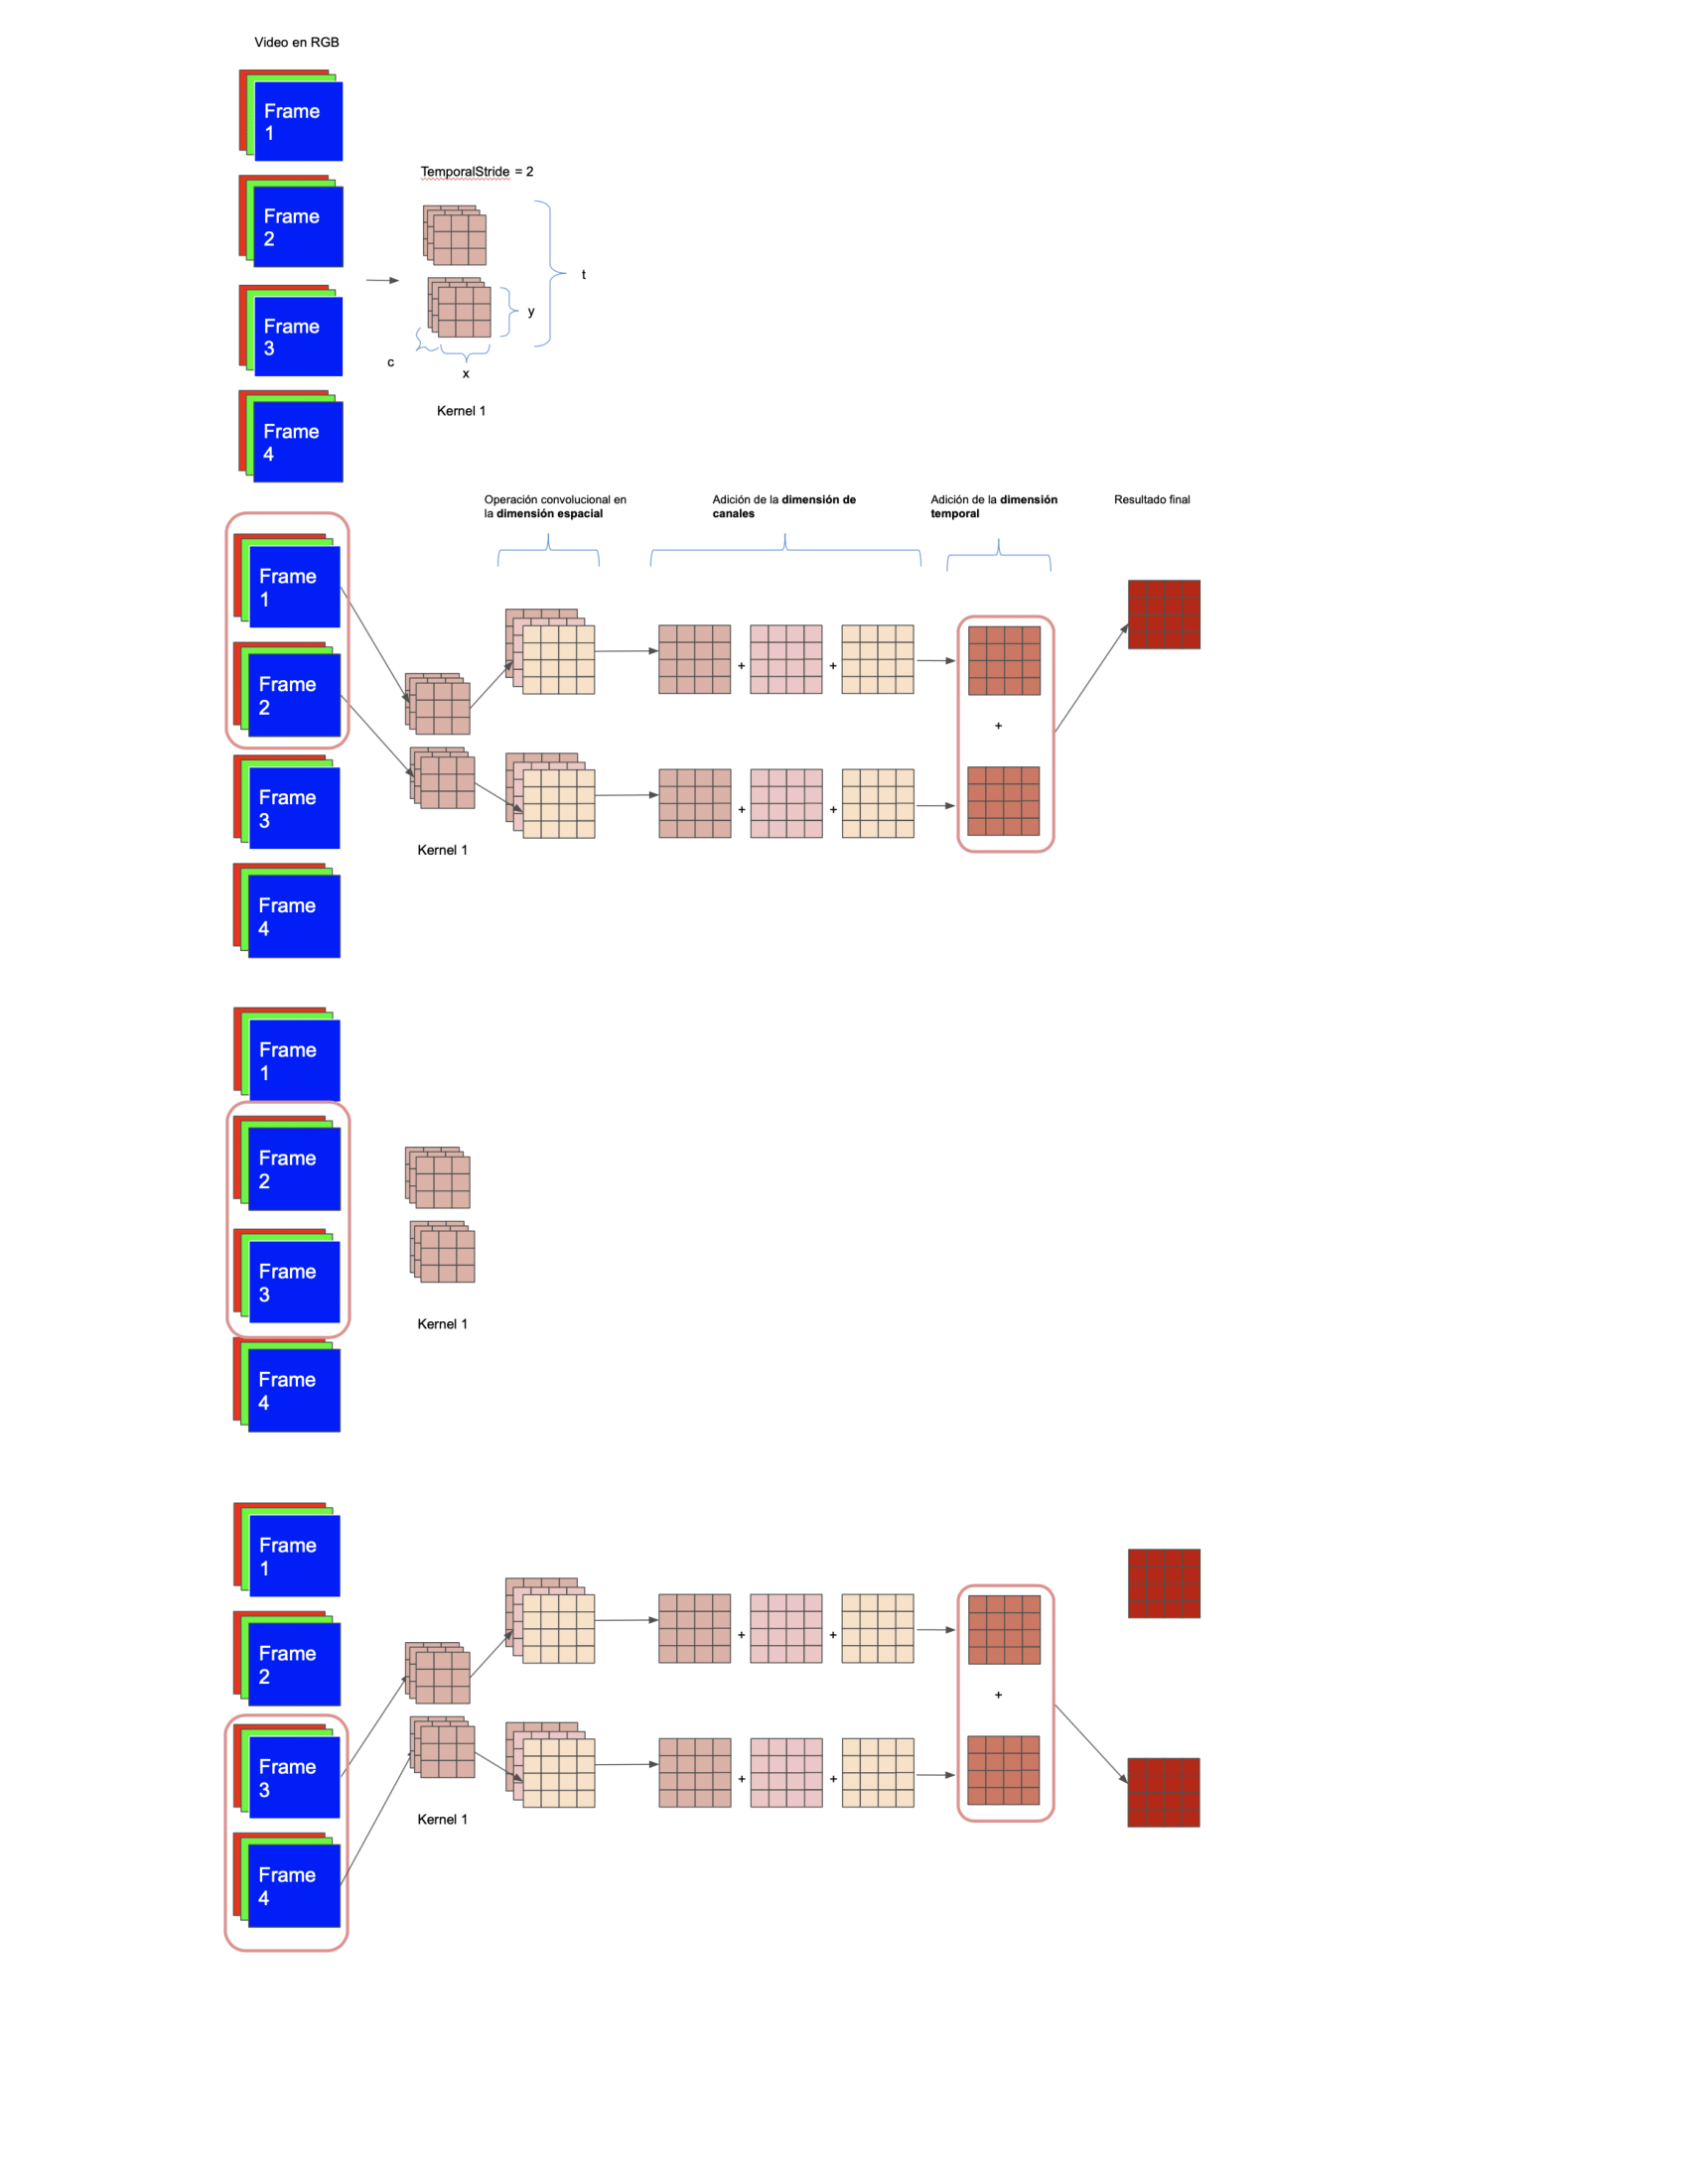
\includegraphics[width=19cm,keepaspectratio]{XX_Figures/Fig_3DCNN_TemporalStride.png}
	\caption{\footnotesize Ejemplo de la Figura \ref{fig:Fig_Ejemplo_3DCNN} con TemporalStride = 2}
	\label{fig:Fig_3DCNN_TemporalStride}
\end{figure}

Se ha demostrado que varias arquitecturas de red 3D CNN son capaces de extraer características espaciotemporales capturando la información del movimiento en de los fotogramas adyacentes en un video \cite{Ji20133DRecognition}. Las redes 2D CNNs previamente analizadas están enfocadas generalmente en analizar imágenes las cuales están en 2 dimensiones (una matriz); aunque estrictamente se encuentran en 3 dimensiones por la profundidad de los canales que pueden llegar a tener, pero comúnmente en la literatura las mencionan como redes neuronales convolucionales 2D por las dos operaciones que se hacen para llegar al resultado final como se observa en la figura \ref{fig:Fig_2D_Dimensiones}. Se agrega una dimensión extra a las redes neuronales convolucionales 3D, esta es la dimensión temporal que en un video representa los diferentes fotogramas que tiene. Un ejemplo de esta nueva dimensión se puede apreciar en el ejemplo de la Figura \ref{fig:Fig_Video}\\


En la Figura \ref{fig:Fig_CNN_2Dvs3D} se puede observar las diferencias entre una 2D CNN y una 3D CNN. En el caso de las 3D CNN los kernels tienen una anchura y una altura que es la encargada de aplicar la operación convolucional a la matriz de píxeles (dimensión espacial) de la misma manera que lo hace una 2D CNN; tiene una profundidad que es igual a la la dimensión de los canales que tienen nuestras matrices (por lo general tres canales: RGB) y se hace la misma operación de adición de la dimensión de canales que en las 2D CNN como se muestra en la Figura \ref{fig:Fig_2D_Dimensiones}. La siguiente dimensión que tienen los kernels en la 3D CNN es la dimensión temporal que como se nota en la Figura \ref{fig:Fig_CNN_2Dvs3D} en la que parecería que cada kernel de la 3D CNN  tiene varios kernels; esta nueva dimensión es la encargada de tomar los datos de varios fotogramas (frames) en los videos y juntarlos en una sola matriz de características.\\ 

En la Figura \ref{fig:Fig_2D_Dimensiones} se muestran las operaciones dimensionales que una 2D CNN hace cuando se tiene un kernel y una imagen con tres canales RGB. Se observa en la Figura \ref{fig:Fig_Ejemplo_3DCNN} las operaciones que hace una red 3D CNN con los mismos hiperparámetros que la 2D CNN de la Figura \ref{fig:Fig_2D_Dimensiones} (un kernel e imágenes en RGB) pero con la diferencia de que se aplican las convoluciones a un video con 4 fotogramas (frames). En el primera parte de la Figura \ref{fig:Fig_Ejemplo_3DCNN} se observan los 4 fotogramas con sus 3 canales respectivos y un kernel con dimensión \textit{(t,c,y,x)} en la que \textit{(y,x) = (3,3)} corresponden al plano espacial, \textit{c = 3} corresponde a la dimensión de los canales (RGB) y \textit{t = 2} corresponde a la dimensión temporal que tiene el kernel. Como la entrada es una cierta cantidad de fotogramas, entonces \textit{t = 2} indica que se aplicará el filtro convolucional a dos fotogramas. En la segunda parte de la \ref{fig:Fig_Ejemplo_3DCNN} se observa que la convolución se aplica para los dos primeros fotogramas (fotograma 1 y fotograma 2) por separado. Se aplica el kernel 1 con el primer fragmento para el fotograma uno y se hace la misma operación convolucional y de adición de las dimensiones de canales que en la 2D CNN; después se aplica el kernel 1 con el segundo fragmento del kernel convolucional y se hace el mismo procedimiento; el resultado de los dos fragmentos del kernel 1 hacen una adición de las matrices resultantes correspondientes al plano temporal y termina el primer paso de la convolución. El segundo paso consiste en deslizar una posición hacia abajo el kernel 3D. Durante en transcurso de este trabajo nos referiremos al deslizamiento temporal como TemporalStride. Una vez aplicado el TemporalStride una posición, se vuelve a aplicar el kernel 1 para el fotograma 2 y fotograma 3, y se vuelva a hacer el mismo procedimiento que en el primer paso para obtener una matriz con características conjuntas del fotograma 2 y 3. Para el último paso se vuelve a aplicar un TemporalStride en una posición y se hace el mismo procedimiento que en los dos pasos anteriores. Al final se habrá obtenido 3 matrices de características que contienen información conjuntas de los 4 fotogramas de entrada y termina la operación convolucional 3D. \\

Las redes convolucionales 3D contienen los mismos atributos que las redes convolucionales 2D, tales como el Stride, Padding (mostrados en el Capítulo \ref{Filtros_espaciales}), la operación Pooling y un Kernel \textit{k = (c,y,x)}, pero a diferencia con las 2D CNN, las 3D CNN contienen un kernel de dimensión \textit{k = (t,c,y,x)}. También contienen un nuevo hiperparámetro el cuál es el paso temporal (TemporalStride) que indica cuántas posiciones en la dimensión temporal se desea que se mueva el kernel. Un ejemplo se observa en la Figura \ref{fig:Fig_3DCNN_TemporalStride} el cuál toma como referencia el ejemplo de la Figura \ref{fig:Fig_Ejemplo_3DCNN} pero con \textit{TemporalStride = 2}.//

La habilidad de analizar series de fotogramas o imágenes en algún contexto le ha dado a las convoluciones 3D varios usos como por ejemplo reconocimiento de acciones \cite{Yang2017DeepImages}; a través de secuencias de imágenes 2D se puede lograr interpretar el movimiento de los objetos para poder predecir ciertas situaciones. También a través del reconocimiento de acciones humanas se ha podido clasificar  los diferentes movimientos que hace un ser humano y con qué objetivo; esto ha sido de gran utilidad para tecnologías que asisten a los humanos, sistemas de seguridad y aplicaciones de realidad virtual. Otro ejemplo en la cual es usada la red 3D CNN es la evaluación de imágenes médicas; estas imágenes se realizan mediante la captura de cortes de la profundidad del tejido a evaluar, combinando estas imágenes estáticas, se ha logrado la identificación de células cancerosas y la evaluación de la salud arterial \cite{Ji20133DRecognition}.\\

El trabajo actual esta enfocado en analizar videos, por lo tanto el uso de la red convolucional 3D es una excelente propuesta para la extracción de características espaciotemporales.

\begin{figure}[th]
	\centering
	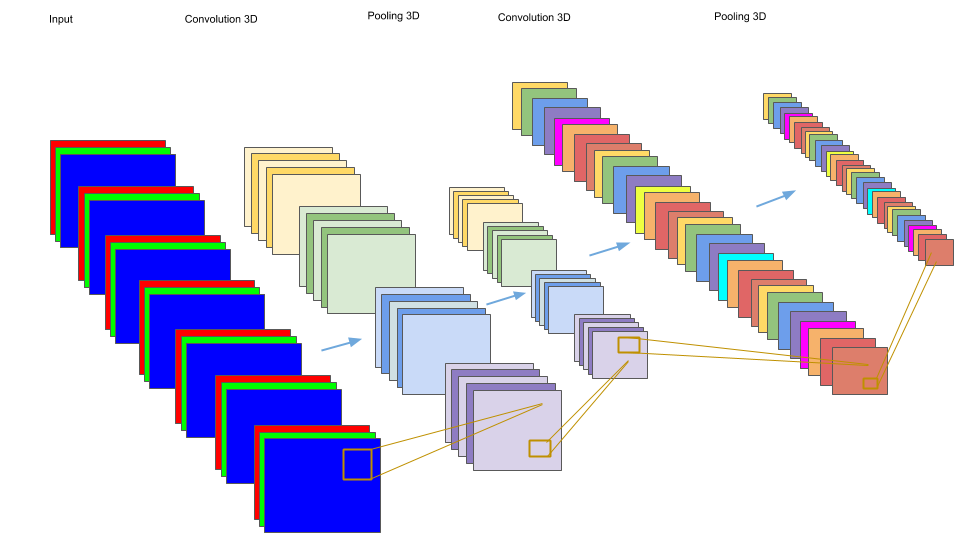
\includegraphics[width=17cm,keepaspectratio]{XX_Figures/Fig_3DCNN_Esquema.png}
	\caption{\footnotesize Esquema de una 3D CNN}
	\label{fig:Fig_3DCNN_Esquema}
\end{figure}

En la Figura \ref{fig:Fig_3DCNN_Esquema}, se muestra un esquema general de las redes neuronales 3D utilizadas para extraer características en videos RGB.


\end{onehalfspacing}